\documentclass[12pt, a4paper, oneside, romanian]{teza-upb}
\setcounter{secnumdepth}{3}
\setcounter{tocdepth}{3}
\usepackage[T1]{fontenc}
\usepackage{babel}
\usepackage{graphicx}
\usepackage{xcolor} % xcolor e mai modern decât color
\usepackage{booktabs} 
\usepackage{tabularx} % Pentru tabele care se auto-ajustează
\usepackage{amsmath}
\usepackage{amssymb}
\usepackage{listings}
\usepackage{color}
\usepackage[
  bookmarks,
  bookmarksopen=true,
  pdftitle={Licenta},
  colorlinks=true,
  allcolors=black,
  linktocpage,
  plainpages=false, 
  pdfpagelabels]{hyperref}
\usepackage{acro}
\usepackage{multicol}
\usepackage{subcaption}
\usepackage{ragged2e}
\usepackage{float}

\singlespacing

% Define abbreviations
\DeclareAcronym{llm}{short = LLM, long = Large Language Model}
\DeclareAcronym{ia}{short = IA, long = Inteligență Artificială}
\DeclareAcronym{rag}{short = RAG, long = Retrieval Augmented Generation}
\DeclareAcronym{api}{short = API, long = Application Programming Interface}
\DeclareAcronym{rca}{short = RCA, long = Root Cause Analysis}
\DeclareAcronym{ci}{short = CI, long = Continuous Integration}
\DeclareAcronym{cd}{short = CD, long = Continuous Deployment}
\DeclareAcronym{e2e}{short = E2E, long = End to End}
\DeclareAcronym{tui}{short = TUI, long = Terminal User Interface}
\DeclareAcronym{oos}{short = OOS, long = Out of Scope}
\DeclareAcronym{mcp}{short = MCP, long = Model Context Protocol}
\DeclareAcronym{lstm}{short = LSTM, long = Long Short Term Memory}
\DeclareAcronym{rnn}{short = RNN, long = Recurrent Neural Network}
\DeclareAcronym{cnn}{short = CNN, long = Convolutional Neural Network}
\DeclareAcronym{btt}{short = BTT, long = Backpropagation Through Time}
\DeclareAcronym{sdd}{short = SDD, long = Spec-Driven Development}
\DeclareAcronym{tdd}{short = TDD, long = Test-Driven Development}
\DeclareAcronym{oss}{short = OSS, long = Open Source Software}
\DeclareAcronym{nlp}{short = NLP, long = Natural Language Processing}
\DeclareAcronym{gpu}{short = GPU, long = Graphics Processing Unit}
\DeclareAcronym{mha}{short = MHA, long = Multi-Head Attention}
\DeclareAcronym{rl}{short = RL, long = Reinforcement Learning}
\DeclareAcronym{kv}{short = KV, long = Key-Value}
\DeclareAcronym{cot}{short = CoT, long = Chain-of-Thought}
\DeclareAcronym{tot}{short = ToT, long = Tree-of-Thought}
\DeclareAcronym{rope}{short = RoPE, long = Rotary Position Embedding}
\DeclareAcronym{json}{short = JSON, long = Java Script Object Notation}
\DeclareAcronym{html}{short = HTML, long = Hyper-Text Markup Language}
\DeclareAcronym{sha}{short = SHA, long = Secure Hash Algorithms}
\DeclareAcronym{pr}{short = PR, long = Pull Request}
\DeclareAcronym{yaml}{short = YAML, long = YAML Ain't Markup Language}
\DeclareAcronym{url}{short = URL, long = Uniform Resource Locator}
\DeclareAcronym{http}{short = HTTP, long = Hyper-Text Transfer Protocol}
\DeclareAcronym{sse}{short = SSE, long = Server-Side Events}
\DeclareAcronym{stdio}{short = STDIO, long = Standard Input-Output}
\DeclareAcronym{posix}{short = POSIX, long = Portable Operating System Interface}
\DeclareAcronym{aml}{short = AML, long = Adversarial Machine Learning}
\DeclareAcronym{cpu}{short = CPU, long = Central Processing Unit}

 
% Define custom colors for code listings
\definecolor{codegreen}{rgb}{0,0.6,0}
\definecolor{codegray}{rgb}{0.5,0.5,0.5}
\definecolor{codepurple}{rgb}{0.58,0,0.82}
\definecolor{backcolour}{rgb}{0.95,0.95,0.92}

% Define custom styles
\lstdefinestyle{mystyle}{
	language=Bash,
    commentstyle=\color{codegreen},
    keywordstyle=\color{blue},
    numberstyle=\tiny\color{codegray},
    stringstyle=\color{codepurple},
	  basicstyle=\ttfamily\scriptsize,
    breakatwhitespace=false,         
    breaklines=true,                 
    captionpos=b,                    
    keepspaces=true,                 
    numbers=left,                    
    numbersep=5pt,                  
    showspaces=false,                
    showstringspaces=false,
    showtabs=false,                  
    tabsize=2
}

\lstdefinelanguage{YAML}{
  keywords={true,false,null,yes,no},
  keywordstyle=\color{blue}\bfseries,
  sensitive=true,
  comment=[l]{\#},
  commentstyle=\color{gray}\itshape,
  stringstyle=\color{red},
  morestring=[b]',
  morestring=[b]",
  literate=
    {---}{{\textcolor{magenta}{---}}}{3}
    {:}{{\textcolor{magenta}{:}}}{1}
    {-}{{\textcolor{magenta}{-}}}{1},
}

% Set custom styles
\lstset{style=mystyle}

\begin{document}

% Variables
\author{Eduard-Daniel NANESCU}
\grupa{441A}
\title{Arhitectură Agentică pentru Asistență Inteligentă în Dezvoltarea Software}
\facultatea{Facultatea de Electronică, Telecomunicații și Tehnologia Informației}
\tiplucrare{licență}
\domeniu{Calculatoare si Tehnologia Informatiei}
\catedra{Electronică Aplicată şi Ingineria Informaţiei}
\campus{Leu}
\program{Ingineria Informatiei}
\titlulobtinut{Inginer}
\director{Ș.L. dr. ing. Mihai DOGARIU}
\directordepartament{Conf. dr. ing Bogdan FLOREA}
\decan{Prof. dr. ing. Mihnea UDREA}
\submissionmonth{Iunie}
\submissionyear{2026}

% Expand variables
\makeatletter

% Set the description of the project as seen on the ETTI website
\renewcommand{\projectdescription} {

  \newpage
  \thispagestyle{empty}

  \noindent

  \begin{minipage}[t]{0.75\textwidth}
    Universitatea Națională de Știință și Tehnologie POLITEHNICA București\\
    Facultatea de Electronică, Telecomunicații și Tehnologia Informației\\
    Program de studiu \textbf{INF}
  \end{minipage}%

  \begin{minipage}[t]{0.25\textwidth}
    \raggedleft
    \textbf{}
  \end{minipage}

  \vspace{1cm}

  \begin{center}
    \textbf{TEMA PROIECTULUI DE DIPLOMĂ}\\
    a studentului \textbf{\@author, \@grupa}
  \end{center}

  \vspace{0.5cm}

  \noindent \textbf{1. Titlul temei:} \@title

  \vspace{0.4cm}

  \noindent \textbf{2. Descrierea temei:}\\
  Contribuția originală a lucrării va consta în dezvoltarea unei arhitecturi software bazată pe Modele Mari de Limbaj (LLMs - Large Language Models), capabilă să asiste utilizatorul în scrierea, depanarea, documentarea și explicarea codului sursă. Aplicațiile vizate sunt eficientizarea procesului de dezvoltare software și automatizarea sarcinilor repetitive întâlnite în programare. Sistemul propus nu vizează antrenarea de la zero a modelelor, ci implementarea unei soluții agentice care utilizează modele pre-antrenate pentru a executa acțiuni complexe. Cercetarea aferentă va include: sinteza bibliografică a realizărilor actuale din domeniu, utilizarea unui mecanism care permite modelului să utilizeze instrumente pentru a interacționa cu mediul virtual, implementarea unor tehnici de inginerie a prompturilor și management-ul contextului pentru a asigura relevanța răspunsurilor, validarea experimentală a prototipului dezvoltat prin scenarii de utilizare reale utilizând medii de dezvoltare precum PyCharm/VS Code și biblioteci specifice precum LangChain, LangGraph sau GoogleADK, concluzionarea rezultatelor obținute și a contribuției originale, cât și enunțarea perspectivelor ulterioare de cercetare.

  \vspace{0.4cm}

  \noindent \textbf{3. Contribuția originală:}\\
  Proiectarea și implementarea arhitecturii agentului, incluzând logica de selecție și utilizare a instrumentelor, gestionarea contextului și dezvoltarea unei interfețe sau integrarea cu interfețe existente care să permită interacțiunea facilă cu asistentul.

  \vspace{0.4cm}

  \noindent \textbf{4. Resurse și bibliografie:}
  \begin{itemize}
    \item Vaswani, Ashish, Noam Shazeer, Niki Parmar, Jakob Uszkoreit, Llion Jones, Aidan N. Gomez, Łukasz Kaiser, and Illia Polosukhin. "Attention is all you need." Advances in neural information processing systems 30 (2017).
    \item Yao, Shunyu, Jeffrey Zhao, Dian Yu, Nan Du, Izhak Shafran, Karthik R. Narasimhan, and Yuan Cao. "React: Synergizing reasoning and acting in language models." In The eleventh international conference on learning representations. 2022.
    \item Bozkurt, Aras, and Ramesh C. Sharma. "Generative AI and prompt engineering: The art of whispering to let the genie out of the algorithmic world." Asian Journal of Distance Education 18, no. 2 (2023): i-vii.
    \item Alto, Valentina. Building LLM Powered Applications: Create intelligent apps and agents with large language models. Packt Publishing Ltd, 2024.
    \item Zhu, He, Tianrui Qin, King Zhu, Heyuan Huang, Yeyi Guan, Jinxiang Xia, Yi Yao et al. "Oagents: An empirical study of building effective agents." arXiv preprint arXiv:2506.15741 (2025).
  \end{itemize}
  \vspace{1.5cm}

  \noindent \textbf{5. Data înregistrării temei:} 2025-12-11 22:54:00

  \vspace{1.5cm}

  \noindent
  \begin{tabular*}{\textwidth}{@{}l@{\extracolsep{\fill}}r@{}}
    \textbf{Conducător(i) lucrare,} & \textbf{Student,} \\
    \@director & \@author \\
    & \\
    & \\
    & \\
    \textbf{Director departament,} & \textbf{Decan,} \\
    \@directordepartament & \@decan
  \end{tabular*}

  \vspace{1.5cm}

  \noindent Cod Validare: \textbf{621d9dfde3}
  \newpage
}

% Don't expand variables
\makeatother

% Template generated content -----------------

\beforepreface

\pagenumbering{arabic}

\listoffigures
\listoftables

\unnumberedsection{LISTA DE ACRONIME}
\begin{multicols}{2}
\printacronyms[heading=none]
\end{multicols}

\newpage
\makeatletter
\afterprefacetrue
\makeatother
\pagestyle{topright}

% --------------------------------------------

\chapter*{INTRODUCERE}
\addcontentsline{toc}{chapter}{INTRODUCERE}

\section*{CONTEXT SI MOTIVATIE}
\addcontentsline{toc}{section}{CONTEXT SI MOTIVATIE}

  Motivatia acestei lucrari vine din experienta personala in industria dezvoltarii software. 
  Atributiile unui inginer software sunt numeroase, diverse si adesea repetitive. Aceasta congestie a timpului ingreuneaza procesul de dezvoltare. 
  A scrie cod a devenit doar o mica parte din sarcinile unui inginer software, pierzand teren in fata design-urilor, 
  documentatiei, review-urilor,
  a testelor unitare de integrare si \ac{e2e}, instrumentarii si monitorizarii, procesului de \ac{ci}/\ac{cd}, 
  infrastructurii, iar in cazul problemelor a debugging-ului si a analizei cauzelor principale (\ac{rca}).
  
  Un inginer software care lucreaza intr-o companie ce deserveste milioane de clienti din intreaga lume trebuie sa fie competitiv, 
  iar aceasta competitivitate se rezuma la a fi la curent cu cele mai noi practici
  din domeniu, cunoasterea notiunilor de programare, securitate cibernetica, retelistica si infrastructura, 
  dar sa si retina simultan informatii vitale despre arhitectura si sistemele interne ale companiei, totul pe langa instruirea colegilor 
  noi sau sedinte.
  
  Timpul unui inginer este astfel impartit de foarte multe procese dinamice care trebuiesc adresate de un angajat capabil sa sustina
  acest ritm alert.
  
  Avand in vedere cele de mai sus, cat si evolutia recenta a sistemelor bazate pe \ac{ia} ce folosesc un \ac{llm} pentru intelegerea
  si generarea de text, era natural ca directia in care dezvoltarea software urma sa se schimbe catre un proces in care
  multe din sarcinile pe care un inginer le-ar fi avut sunt acum delegate sistemelor automate. Astfel, atentia inginerului se muta 
  de la a scrie cod, la supravegherea instrumentelor de programare bazate pe inteligenta artificiala si asumarea deciziilor arhitecturale.
  Restul grijilor cotidiene pot fi abordate de aceste instrumente, eliberand programul operatorului.
  
  Trecerea de la o experienta pur conversationala cu aceste modele la intrebuintari pentru cautare prin
  limbaj natural, iar in final integrandu-se cu mediile de dezvoltare software si cu terminalul sistemului de operare pentru
  a avea acces la un context mai bun dar si pentru executia de comenzi, nu a fost una dificila, avand in vedere competentele avansate de
  prelucrare si generare de text ale acestor modele.

  Momentan, in domeniul modelelor de limbaj, exista cativa jucatori mari precum Google, Anthropic si OpenAI care controleaza o buna parte
  din cota de piata. Acestia sunt in stadiul in care isi fortifica ecosistemul pentru a-si maximiza retentia de utilizatori. Fiecare furnizor
  de astfel de servicii lanseaza produse care se folosesc de aceste modele. De la asistenti de cercetare, la asistenti de programare si la programe
  ce automatizeaza sarcini zilnice. Odata cu aceste produse, incearca sa restrictioneze sau sa ofere tarife diferite pentru utilizatori ce folosesc
  modelele pentru astfel de sarcini in afara ecosistemului lor.

  Exista si modele de limbaj de tipul \ac{oss}, de diferite marimi si cu diverse proprietati, dar ecosistemul uneltelor gratuite sau \ac{oss} care folosesc aceste modele
  pentru sarcini avansate inca este in proces de dezvoltare. Astfel, este un mediu propice pentru un produs ce livreaza un asistent inteligent pentru dezvoltarea software,
  independent de furnizor, construit pentru costuri reduse, performanta ridicata, abordarea problemelor complexe ce poate rula local, precum cel pe care imi propun sa il realizez in aceasta lucrare.

\section*{SCOPUL SI OBIECTIVELE LUCRARII}
\addcontentsline{toc}{section}{SCOPUL SI OBIECTIVELE LUCRARII}

  Scopul acestei lucrari este de a realiza un \textbf{asistent inteligent extensibil si transparent} bazat pe \ac{ia}, \textbf{agnostic fata de platforma sau de furnizori de modele de limbaj},
  ce ruleaza local sau in cloud si ce poate interactiona cu mediul virtual in care ruleaza (sistem de operare, mediu de dezvoltare,
  internet) prin intermediul uneltelor (
    tool-uri
    \footnote{In \ac{ia} folosita cu ajutorul agentilor \textbf{tool}-urile sunt functii cu descrieri detaliate 
    de folosire pe care agentul le populeaza cu parametrii, le executa si receptioneaza raspunsul pentru 
    a-l folosi mai departe in rezolvarea problemelor complexe}), realizat de un workflow agentic
    \footnote{\textbf{Agentii} sunt aplicatii ce folosesc inteligenta artificiala pentru a interactiona cu mediul inconjurator}

  Obiectivul principal care trebuie atins este realizarea unui produs functional ce poate ajuta un inginer software in cat mai multe aspecte ale meseriei sale.
  Pentru a indeplini acest obiectiv, trebuie sa avem in vedere urmatoarele necesitati: interfata facila ce poate fi folosita oriunde folosind terminalul
  sistemului de operare (\ac{tui}), suficiente unelte pentru a indeplini sarcini cat mai complexe, management-ul conversatiei, contextului si al memoriei,
  versionare, evaluari si teste de regresie, monitorizare si observabilitate (metrici), siguranta (medii sigure pentru executarea codului,
  masuri de protectie pentru date de intrare malitioase, \ac{oos} detection), si cel mai important: un prompt de sistem ales cu grija.

\newpage


\chapter{LUCRARI ANTERIOARE}

  O buna intelegere a tehnologiilor, standardelor si a obstacolelor actuale din industrie necesita
  studierea literaturii de specialitate, a lucrarilor si a arhitecturilor existente deja in domeniu. Acest pas este
  obligatoriu pentru alegeri informate in cadrul implementarii proiectului, evitarea problemelor deja recunoscute 
  si confera o vedere de ansamblu asupra stadiului final al lucrarii.

  \section{Evolutia catre modelele mari de limbaj (\ac{llm})}

  Domeniul inteligentei artificiale a fost studiat o perioada indelungata iar cateva publicatii au marcat industria
  prin concepte revolutionare si progrese importante.

  Unul din conceptele de baza ale inteligentei artificiale a aparut pentru prima data publicat in anul 1958 de catre F. Rosenblatt in lucrarea \cite{rosenblattPerceptronProbabilisticModel1958}, 
  unde este prezentat \textbf{perceptronul}: un model inspirat din fizionomia neuronului biologic, capabil sa realizeze sarcini de clasificare binara. Perceptronul primeste un set de date
  de intrare, fiecare asociata unei ponderi, iar rezultatul final este determinat prin combinarea acestor valori si aplicarea unei functii de activare. Procesul de invatare
  are loc prin ajustarea iterativa aponderilor in functie de eroarea obtinuta la iesire, mecanism ce reprezinta baza invatarii automate moderne. Aceasta abordare a demonstrat pentru prima data
  posibilitatea construirii unor sisteme capabile sa invete din experienta, fara a fi programate explicit pentru fiecare situatie (Figura~\ref{fig:perceptron}).

  Formal, pentru un vector de intrare $\mathbf{x} \in \mathbb{R}^{n}$, un vector de ponderi $\mathbf{w} \in \mathbb{R}^{n}$ si un termen de prag $b$, iesirea perceptronului este data de:
  \begin{equation}
    y = \varphi\!\left( \sum_{i=1}^{n} w_i\, x_i + b \right) = \varphi(\mathbf{w}^{\top}\mathbf{x} + b),
    \label{eq:perceptron}
  \end{equation}
  unde $\varphi(\cdot)$ este functia de activare (treapta in formularea originala). Regula de invatare consta in actualizarea ponderilor proportional cu eroarea $e = y_{\text{tinta}} - y$ si cu o rata de invatare $\eta$, $\mathbf{w} \leftarrow \mathbf{w} + \eta\, e\, \mathbf{x}$.

  Cu toate acestea, desi perceptronul a reprezentat un pas revolutonar in dezvoltarea inteligentei artificiale, modelul prezenta limitari importante. In forma sa initiala,
  acesta putea clasifica doar date liniar separabile, ceea ce restrictiona capacitatea de rezolvare a problemelor complexe. Din acest motiv, perceptronul simplu era eficient doar pentru reprezentari de
  date de intrare relativ simple, intr-un singur strat de procesare. Aceste limitari au dus ulterior la dezvoltarea retelelor neuronale multistrat si a algoritmilor mai avansati de antrenare, care au stat la
  baza progreselor moderne din domeniul inteligentei artificiale.

  \begin{figure}[htbp]
    \centering
    \includegraphics*[width=0.4\columnwidth]{figuri/perceptron.png}
    \caption{Modelul unui perceptron (\href{https://jretamales.github.io/2019-01-29-embeddings_101}{sursa})}
    \label{fig:perceptron}
  \end{figure}
  

  Un progres major s-a ivit odata cu introducerea retelelor neurale convolutionale (\ac{cnn}) de catre Yann LeCun si colaboratorii sai in lucrarea \cite{lecunGradientbasedLearningApplied1998}.
  Aceasta abordare a fost conceputa pentru a depasi limitarile modelelor anterioare, precum perceptronul simplu care nu putea procesa eficient informatii
  complexe din imagini. Aparitia retelelor convolutionale a marcat inceputul aplicarii pe scara larga a inteligentei artificiale in domeniul procesarii si analizei imaginilor.

  Ideea fundamentala din spatele acestor retele era relativ rudimentara, insa extrem de eficienta: datele de intrare nu mai sunt tratate ca pe un vector unidimensional, astfel
  modelul analiza portiuni locale ale imaginii prin intermediul unor "ferestre" de convolutie. Aceste filtre parcurg imaginea si extrag automat trasaturi relevante, precum muchii,
  forme sau texturi. In plus, utilizarea mai multor straturi succesive permitea retelei sa invete reprezentari din ce in ce mai abstracte si mai complexe
  ale datelor vizuale.

  Un alt element important introdus de retelele convolutionale a fost utilizarea operatiilor specializate, precum convolutia (Figura~\ref{fig:convolutie}) si subsampling-ul (pooling), care reduceau
  dimensionalitatea datelor si imbunatateau capacitatea de generalizare a modelului. Astfel, \ac{cnn} au devenit capabile sa identifice tipare spatiale
  complexe si sa obtina performante superioare in sarcini precum recunoasterea faciala, clasificarea imaginilor sau detectia obiectelor. Aceste inovatii au reprezentat
  fundamentul dezvoltarii ulterioare a tehnologiilor moderne de computer vision si deep learning.

  \newpage

  \begin{figure}[htbp]
    \centering
    \includegraphics*[width=0.8\columnwidth]{figuri/convolutie.png}
    \caption{Convolutia cu un nucleu a unei imagini (\href{https://www.geeksforgeeks.org/deep-learning/kernels-filters-in-convolutional-neural-network/}{sursa})}
    \label{fig:convolutie}
  \end{figure}

  Desi retelele neurale convolutionale (\ac{cnn}) au demonstrat performante remarcabile in procesarea datelor statice, precum imaginile,
  acestea nu erau potrivite pentru aplicatii in care informatia are caracter secvential. Domenii precum procesarea limbajului natural (\ac{nlp}),
  recunoasterea vorbirii sau analiza datelor in timp presupun existenta unei dependente intre elementele succesive ale datelor, informatia desfasurandu-se
  in timp si nu intr-o structura fixa bidimensionala. Din acest motiv, utilizarea unor "ferestre" locale nu era suficienta pentru captarea relatiilor
  pe termen lung dintre elementele unei secvente.

  Primele incercari de rezolvare a acestei probleme au fost realizate prin intermediul retelelor neuronale recurente (\ac{rnn}), arhitecturi capabile sa
  pastreze informatia din pasii anteriori prin intermediul unei stari interne. Astfel, modelul putea utiliza contextul anterior pentru a influenta predictiile curente, ceea ce
  reprezenta un progres important pentru procesarea datelor temporale. Cu toate acestea, antrenarea \ac{rnn} clasice s-a confruntat rapid cu o problema fundamentala a invatarii
  profunde: disparitia gradientului.

  Aceasta problema aparea in timpul procesului de propagare inversa prin timp (\ac{btt}), atunci cand secventele analizate deveneau foarte lungi.
  Gradientii calculati in timpul antrenarii se diminuau exponential pe masura ce informatia era propagata catre inceputul secventei, devenind atat de mici incat actualizarile ponderilor
  ajungeau neglijabile. In consecinta, reteaua "uita" informatiile importante del a inceputul secventei si nu putea invata \textit{dependente pe termen lung}.

  Un progress major a fost realizat de Sepp Hochreiter si Jürgen Schmidhuber prin introducerea arhitecturii \ac{lstm} in lucrarea 
  \cite{hochreiterLongShortTermMemory1997}. Acest model a oferit retelelor neuronale o forma functionala de memorie pe termen lung, capabila sa pastreze
  informatii relevante pentru perioade extinse de timp. Elementul central al acestei arhitecturi il reprezinta mecanismul de "porti" care controleaza
  fluxul informatiei in interiorul retelei. Prin aceste mecanisme, modelul poate decide ce informatii trebuie pastrate, ce informatii trebuie actualizate
  si ce informatii trebuie eliminate din memorie.

  Datorita acestei capacitati de gestionare eficienta a contextului temporal, retelele \ac{lstm} au devenid fundamentul multor
  aplicatii moderne de inteligenta artificiala, fiind utilizate cu succes in traducere automata, recunoastere vocala, generare de text
  si analiza de secvente temporale, desi problema disparitiei gradientilor nu disparuse complet. O comparatie schematica intre cele doua arhitecturi este prezentata in Figura~\ref{fig:rnn-lstm}.

  La pasul de timp $t$, dinamica unei celule \ac{lstm} poate fi descrisa prin trei porti (uitare, intrare si iesire) si o stare de celula $\mathbf{c}_t$:
  \begin{equation}
    \begin{aligned}
      \mathbf{f}_t &= \sigma(\mathbf{W}_f [\mathbf{h}_{t-1}, \mathbf{x}_t] + \mathbf{b}_f), \\
      \mathbf{i}_t &= \sigma(\mathbf{W}_i [\mathbf{h}_{t-1}, \mathbf{x}_t] + \mathbf{b}_i), \\
      \mathbf{o}_t &= \sigma(\mathbf{W}_o [\mathbf{h}_{t-1}, \mathbf{x}_t] + \mathbf{b}_o), \\
      \mathbf{c}_t &= \mathbf{f}_t \odot \mathbf{c}_{t-1} + \mathbf{i}_t \odot \tanh(\mathbf{W}_c [\mathbf{h}_{t-1}, \mathbf{x}_t] + \mathbf{b}_c), \\
      \mathbf{h}_t &= \mathbf{o}_t \odot \tanh(\mathbf{c}_t),
    \end{aligned}
    \label{eq:lstm}
  \end{equation}
  unde $\sigma$ este functia sigmoid, $\odot$ produsul Hadamard, iar $[\cdot,\cdot]$ desemneaza concatenarea vectorilor. Stocarea informatiei in $\mathbf{c}_t$ printr-o cale aditiva (controlata de $\mathbf{f}_t$ si $\mathbf{i}_t$) este principalul motiv pentru care gradientii nu se diminueaza la fel de rapid ca in cazul unei \ac{rnn} clasice.

  \begin{figure}[htbp]
    \centering
    \begin{subfigure}[b]{0.48\textwidth}
      \centering
      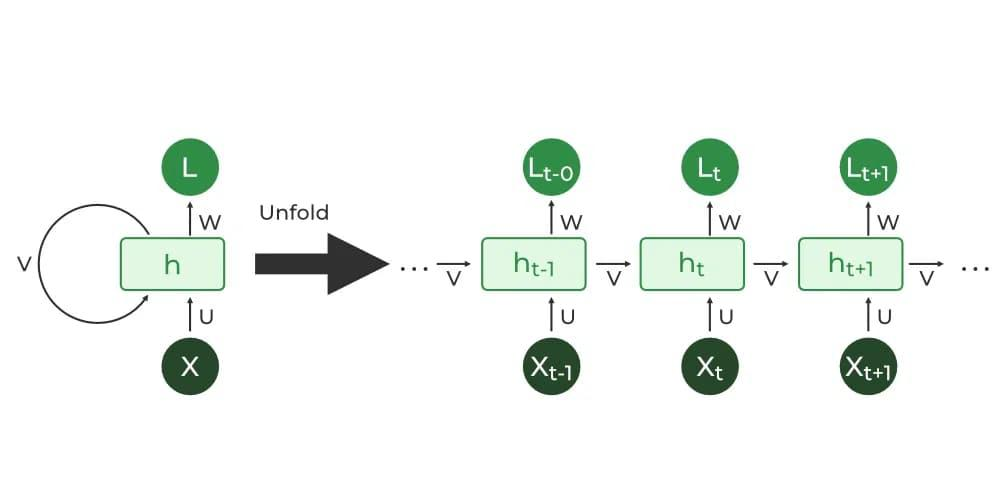
\includegraphics[width=\linewidth]{figuri/rnn.png}
      \caption{\ac{rnn}}
      \label{fig:rnn}
    \end{subfigure}
    \hfill
    \begin{subfigure}[b]{0.48\textwidth}
      \centering
      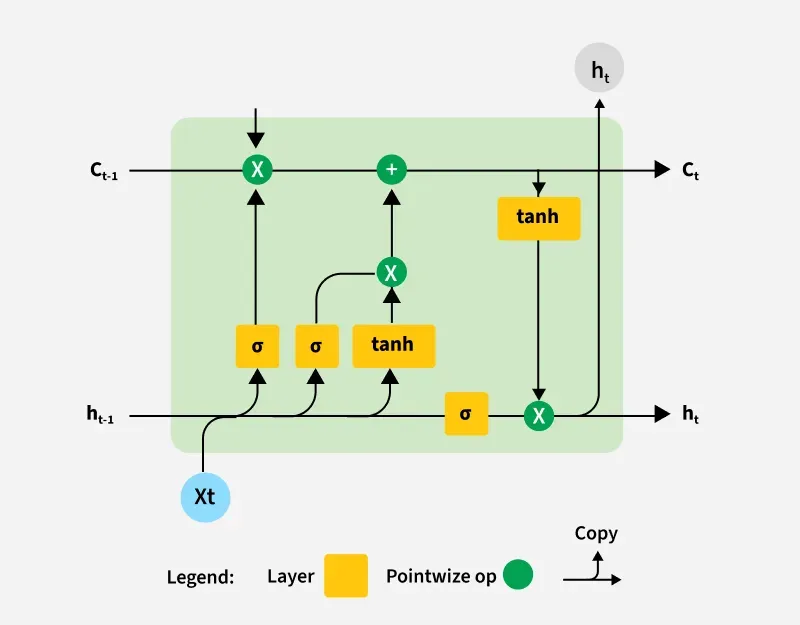
\includegraphics[width=\linewidth]{figuri/lstm.png}
      \caption{\ac{lstm}}
      \label{fig:lstm}
    \end{subfigure}
    \caption{\ac{rnn} si \ac{lstm} comparate (\href{https://www.geeksforgeeks.org/deep-learning/types-of-neural-networks/}{sursa})}
    \label{fig:rnn-lstm}
  \end{figure}

  \textbf{Punctul de cotitura in evolutia inteligentei artificiale} a fost reprezentat de introducerea arhitecturii "transformer", prezentata
  de Vaswani si colaboratorii sai in lucrarea devenita celebra \cite{vaswaniAttentionAllYou2017}. Pana in acel moment, modelele bazate pe 
  \ac{lstm} dominau procesarea limbajului natural, insa acestea prezentau o limitare importanta: datele secventiale trebuiau procesate pas cu pas,
  fiecare element depinzand de rezultatul precedent. Aceasta caracteristica facea antrenarea pe volume foarte mari de date sa fie lenta si dificil
  de paralelizat, limitand scalabilitatea modelelor.

  Arhitectura transformer (Figura~\ref{fig:transformer}) a schimbat fundamental aceasta abordare prin introducerea mecanismului de \textbf{self-attention}. In loc sa proceseze secvential,
  modelul putea analiza simultan toate elementele unei propozitii si putea calcula relatiile dintre aceastea indiferent de distanta lor intext.
  Astfel, fiecare cuvant primea informatii contextuale din intreaga secventa, ceea ce permitea captarea mult mai eficienta a dependentelor
  semantice si sintactice. In plus, eliminarea procesarii strict secventiale a permis paralelizarea operatiilor pe hardware modern precum \ac{gpu}, 
  reducand seminifcativ timpul de antrenare.

  Mecanismul de \textit{scaled dot-product attention} este definit, pentru matricile de interogari $\mathbf{Q} \in \mathbb{R}^{n \times d_k}$, chei $\mathbf{K} \in \mathbb{R}^{n \times d_k}$ si valori $\mathbf{V} \in \mathbb{R}^{n \times d_v}$, prin:
  \begin{equation}
    \mathrm{Attention}(\mathbf{Q}, \mathbf{K}, \mathbf{V}) = \mathrm{softmax}\!\left( \frac{\mathbf{Q}\mathbf{K}^{\top}}{\sqrt{d_k}} \right) \mathbf{V},
    \label{eq:attention}
  \end{equation}
  unde factorul $1/\sqrt{d_k}$ stabilizeaza gradientii pentru valori mari ale dimensiunii cheilor.

  Mai tarziu, mecanismul de "self-attention" s-a transformat in "multi-head attention" care avea cate un cap de atentie pentru caracteristici specifice, putand astfel
  sa invete multiple tipuri de dependente intre date, fiecare cap specializandu-se pe un anumit tip mai mult sau mai putin abstract de dependenta intre date. Pe langa deblocarea
  intelegerii relatiilor complexe, \ac{mha} a adus si o optimizare in timpul de antrenare si de inferenta, dar si la imbunatatirea generalizarii modelelor. Formal, pentru $h$ capete de atentie:
  \begin{equation}
    \begin{aligned}
      \mathrm{MultiHead}(\mathbf{Q}, \mathbf{K}, \mathbf{V}) &= \mathrm{Concat}(\mathrm{head}_1, \dots, \mathrm{head}_h)\, \mathbf{W}^{O}, \\
      \mathrm{head}_i &= \mathrm{Attention}(\mathbf{Q}\mathbf{W}_i^{Q}, \mathbf{K}\mathbf{W}_i^{K}, \mathbf{V}\mathbf{W}_i^{V}),
    \end{aligned}
    \label{eq:mha}
  \end{equation}
  cu matricile de proiectie $\mathbf{W}_i^{Q}, \mathbf{W}_i^{K} \in \mathbb{R}^{d_{\text{model}} \times d_k}$, $\mathbf{W}_i^{V} \in \mathbb{R}^{d_{\text{model}} \times d_v}$ si $\mathbf{W}^{O} \in \mathbb{R}^{h d_v \times d_{\text{model}}}$.

  \newpage

  \begin{figure}[htbp]
    \centering
    \includegraphics*[width=0.4\columnwidth]{figuri/transformer.png}
    \caption{Arhitectura transformer \cite{vaswaniAttentionAllYou2017}}
    \label{fig:transformer}
  \end{figure}

  Odata eliminata limitarea din punct de vedere computational, cercetatorii au putut antrena modele pe seturi de date de dimensiuni fara precedent.
  Acest progres a deschis drumul catre aparitia modelelor mari de limbaj, \ac{llm}. Acestea sunt capabile sa invete reprezentari complexe ale
  limbajului natural prin analizarea unor cantitati uriase de text provenite din carti, articole, pagini web si alte surse disponibile pe internet.
  Transformerul a devenit rapid fundamentul majoritatii sistemelor moderne de inteligenta artificiala dedicate limbajului natural, influentand profund atat cercetarea academica,
  cat si aplicatiile comerciale.

  Modelele mari de limbaj reprezinta rezultatul direct al antrenarii retelelor pe volume masive de date si folosind un numar foarte mare de parametrii.
  Cercetatorii au observat ca performanta modelelor continua sa creasca odata cu extinderea dimensiunii acestora si a cantitatii de date
  utilizate la antrenare. Pornind de la aceasta idee, echipa OpenAI a dezvoltat modelul GPT-3, care includea aproximativ \textbf{175 de miliarde de parametrii}, descoperirile fiind prezentate in lucrarea „Language Models are Few-Shot Learners” \cite{brownLanguageModelsAre2020a}. La momentul
  aparitiei, GPT-3 reprezenta unul dintre cele mai mari si mai performante modele lingvistice create.

  Una din cele mai importante realizari ale acestui model a fost capacitatea de a rezolva sarcini complexe fara a necesita o antrenare
  suplimentara specifica fiecarei probleme. Prin simpla furnizare a catorva exemple sau chiar doar a unei instructiuni formulate in limbaj natural,
  modelul putea genera cod sursa, realza sumarizari de text, raspunde la intrebari, traduce texte sau crea continut creativ precum poezii si eseuri. Aceasta
  particularitate a fost documentata in articolul prezentat anterior a demonstrat ca modelele de mari dimensiuni pot generaliza cunostiinte intre domenii diferite si
  isi pot adapta comportamentul fara modificari suplimentare ale parametrilor interni.

  Prin aceste progrese, inteligenta artificiala a facut tranzitia de la sisteme specializate, concepute pentru rezolvarea unei sarcini predefinite, la
  modele capabile sa manifeste competente generale avansate. Aceasta schimbare a reprezentat inceputul unei noi etape in dezvoltarea inteligentei artificiale moderne,
  in care accentul s-a mutat de la proiectarea unor solutii dedicate catre construirea unor modele inteligente universal, capabile
  sa interactioneze natural cu oamenii si sa rezolve probleme complexe.

  \section{Maturizarea modelelor mari de limbaj si cercetari actuale}

  Odata cu aparitia primelor foundation models
  \footnote{Un foundation model este un model mare de limbaj de uz general antrenat pe cantitati foarte mari date diverse,
  ce poate fi adaptat pentru un numar mare de intrebuintari} 
  precum GPT-4, GPT-5, Sonnet sau Opus, industria inteligentei artificiale a cunoscut o crestere exponentiala. Aceste modele
  prezinta o eficacitate impresionanta in rezolvarea problemelor din domenii diverse, de la generare si analiza textului, pana la
  programare, traduceri automate, automatizari complexe sau gandire logica. Datorita acestei flexibilitati, integrarea acestor modele
  a devenit o prioritate pentru majoritatea companiilor ce activau in domeniul tehnologiei.
  
  \begin{figure}[H]
    \centering
    \includegraphics*[width=0.8\columnwidth]{figuri/evolutie_ai.png}
    \caption{Evolutia recenta a modelelor mari de limbaj \cite{zhaoSurveyLargeLanguage2026}}
    \label{fig:evolutia_ai}
  \end{figure}

  Astfel, cresterea rapida a cererii pentru sisteme bazate pe inteligenta artificiala a determinat furnizorii de astfel de modele si alte
  companii care ar beneficia de pe urma modelelor, sa investeasca masiv in cercetare si infrastructura. Aceste investitii au permis in final
  antrenarea unor modele cu capacitati din ce in ce mai sofisticate, fiecare noua generatie de modele aducand imbunatatiri semnificative
  in ceea ce priveste rationamentul, intelegerea limbajului si capacitatea de a rezolva probleme complexe.

  \begin{figure}[H]
    \centering
    \includegraphics*[width=0.8\columnwidth]{figuri/evolutie_open_ai.png}
    \caption{Evolutia modelelor GPT \cite{zhaoSurveyLargeLanguage2026}}
    \label{fig:evolutia_open_ai}
  \end{figure}

  Investitiile in infrastructura nu au fost singurul motiv pentru care modelele de limbaj au avut o crestere impresionanta. Cercetarea
  a jucat de asemenea un rol crucial in optimizarea lor. Multe optimizari au fost aduse acestor modele de limbaj, printre care
  si imbunatatiri ale arhitecturii transformer care isi propun optimizeze modelele pentru procesarea secventelor mai lungi de date de intrare, precum
  este ilustrat in lucrarea "Longformer: The Long-Document Transformer" \cite{beltagy_longformer_2020-1} de Beltagy si colaboratorii sai care isi propun
  sa optimizeze mecanismul de atentie, folosind serii trigonometrice pentru a stabiliza compresia cache-ului \ac{kv}
  \footnote{Un token reprezinta datele de intrare pentru arhitectura transformer si uzual sunt cuvinte, parti din cuvinte sau caractere. Acestea permit modelului sa sparga un cuvant posibil mai rar in parti mai cunoscute.}
  \footnote{Cache-ul \ac{kv} este o optimizare fundamentala a arhitecturii transformer ce elimina calculele redundante ale token-urilor anterioare in generarea autoregresiva, conform lucrarii "KV Cache Optimization Strategies for Scalable and Efficient LLM Inference" de Xu si colaboratorii \cite{xu_kv_2026}}
  imbunatatind astfel gandirea pe termen lung, lucru documentat in lucrarea "TriAttention: Efficient Long Reasoning with Trigonometric KV Compression" de Mao si colaboratorii sai \cite{mao_triattention_2026}.

  \begin{figure}[H]
    \centering
    \includegraphics*[width=0.8\columnwidth]{figuri/longformer1.png}
    \caption{Performanta tipurilor de arhitecturi de tipul "Longformer" \cite{beltagy_longformer_2020-1}. 
    In timp ce mecanismul tipic de atentie utilizeaza memorie exponential, arhitectura Longformer foloseste memorie liniar
    odata cu cresterea contextului}
    \label{fig:longformer1}
  \end{figure}

  \begin{figure}[H]
    \centering
    \includegraphics*[width=0.8\columnwidth]{figuri/longformer2.png}
    \caption{Diferite configuratii de atentie folosite in arhitectura Longformer in comparatie cu mecanismul obisnuit de atentie \cite{beltagy_longformer_2020-1}}
    \label{fig:longformer2}
  \end{figure}

  Inca un punct de optimizare al arhitecturii curente este imbunatatirea embedding-urilor,
  \footnote{Embedding-ul este transformarea token-ului intr-un vector abstract multi-dimensional ce reprezinta informatia extrasa de model din acel token, plus un vector ce aduce informatii despre pozitia acestui in secventa.}
  precum studiul realizat in lucrarea "RoFormer: Enhanced Transformer with Rotary Position Embedding" \cite{su_roformer_2023-1} care isi propune sa optimizeze pozitia exacta a token-ului in secventa cu o matrice de rotatie in 
  timp ce incorporeaza dependenta pozitiei relative in formula mecanismului de atentie, reusind astfel sa capteze informatii importante din secventa de intrare precum, lungimea secventei, relatiile intre tokens care se diminueaza pe masura ce distanta relativa dintre ei creste,
  echipand astfel mecanismul de atentie cu o codare pozitionala relativa.

  \begin{figure}[H]
    \centering
    \includegraphics*[width=0.8\columnwidth]{figuri/roformer.png}
    \caption{Principiul de baza pentru \ac{rope} \cite{su_roformer_2023-1}}
    \label{fig:roformer}
  \end{figure}

  Imbunatatiri s-au adus si in partea de fine-tuning
  \footnote{Fine tuning-ul este un procedeu prin care parametrii unui model sunt ajustati pentru eficienta sporita intr-un anumit domeniu.}
  mai ales prin lucrarea LoRA: Low-Rank Adaptation of Large Language Models" \cite{huLoRALowRankAdaptation2021} care aduce imbunatatiri prin inghetarea ponderilor modelului
  si injectarea unor matrici antrenabile de descompunere in fiecare strat al arhitecturii transformer, reducand numarul de parametrii antrenabili, reducand numarul acestor de \textbf{pana la 10.000 de ori}
  si puterea de calcul necesara de \textbf{3 ori} in comparatie cu fine-tuning-ul normal. Concret, pentru o matrice de ponderi pre-antrenata $\mathbf{W}_0 \in \mathbb{R}^{d \times k}$, actualizarea este aproximata printr-o descompunere de rang mic:
  \begin{equation}
    \mathbf{W} = \mathbf{W}_0 + \Delta\mathbf{W} = \mathbf{W}_0 + \mathbf{B}\mathbf{A}, \qquad \mathbf{B} \in \mathbb{R}^{d \times r},\; \mathbf{A} \in \mathbb{R}^{r \times k},\; r \ll \min(d, k),
    \label{eq:lora}
  \end{equation}
  unde doar $\mathbf{A}$ si $\mathbf{B}$ sunt antrenate, in timp ce $\mathbf{W}_0$ ramane inghetata.

  \begin{figure}[H]
    \centering
    \includegraphics*[width=0.4\columnwidth]{figuri/lora.png}
    \caption{Fine-tuning-ul se realizeaza doar pe A si B \cite{huLoRALowRankAdaptation2021}}
    \label{fig:lora}
  \end{figure}

  Performanta a vazut de asemenea progrese, spre exemplu prin procedeul de decodare speculativa prezentata in articolul "Fast Inference from Transformers via Speculative Decoding" \cite{leviathanFastInferenceTransformers2023}
  care ilustreaza problema timpului de inferenta
  \footnote{Inferenta este procedeul prin care un model de limbaj ia datele de intrare, aplica transformarile necesare si produce un raspuns final.}
  care continua sa creasca pe masura ce marimea modelelor creste si ea. Autorii propun un algoritm care sa permita livrarea mai multor tokeni in paralel. La baza lucrarii stau doua observatii funamentale:
  (1) majoritatea sarcinilor abordate de modelele mari de limbaj pot fi scindate in obiective mai usoare care pot fi abordate de modele mai eficiente si (2) folosind executia speculativa si o noua metoda de esantionare, decodarea
  poate fi accelerata rulandu-le in paralel pe baza iesirilor modelele mai eficiente ce aproximeaza pe cat de bine pot, generand mai multi tokeni simultan fara a modifica distributia.

  Continuand incercarile de a eficientiza modelele mari de limbaj, a aparut intrebarea: "Daca marimea modelul incetineste antrenarea si inferenta, de ce nu cautam sa micsoram modelul?".
  Astfel, au aparut procedeele de cuantizare
  \footnote{Cuantizarea este reducerea tipului de date care stocheaza parametrii retelei. Spre exemplu daca in loc de 8 biti, stocam parametrii pe 4 biti, injumatatim amprenta modelului}
  si distilare
  \footnote{Distilarea este antrenarea unui model mai mic prin obiectivul reproducerii raspunsurilor modelului mai mare}. Problema distilarii este nevoia unui model superior care sa poarte rolul
  de "invatator". Zhang si echipa sa de cercetatori documenteaza o alternativa a acestei metode prin procedeul de distilare proprie in lucrarea "Embarrassingly Simple Self-Distillation Improves Code Generation"
  \cite{zhang_embarrassingly_2026-2} prin esantionarea cu anumite valori ale temperaturii 
  \footnote{Temperatura este o setare pentru modelele de limbaj care controleaza "creativitatea" modelului. O temperatura mica (spre exemplu 0) obliga modelul sa scoata la iesirea sa 
  cel mai probabil token posibil, pe cand o temperatura mare (spre exemplu 0.9), permite modelului sa aleaga un alt token probabil.}
  si configuratii ale trunchierii, in final executand fine-tuning supervizat
  \footnote{Supervizarea se refera la abilitatea modelului de a folosi exemple etichetate corect de oameni in prealabil pentru antrenare. Antrenarea supervizata nu include raspunsurile corecte, iar modelul trebuie sa descopere singur tiparele ce reprezinta raspunsul corect}
  pe acele esantioane. 

  \begin{figure}[H]
    \centering
    \includegraphics*[width=0.8\columnwidth]{figuri/embarr1.png}
    \caption{Rezultatele procesului de Simple Self Distillation \cite{zhang_embarrassingly_2026-2}}
    \label{fig:embarr1}
  \end{figure}

  \begin{figure}[H]
    \centering
    \includegraphics*[width=0.8\columnwidth]{figuri/embarr3.png}
    \caption{Imbunatatiri in sarcini de programare ale modelelor dupa ce au fost supuse procesului de Simple Self Distillation\cite{zhang_embarrassingly_2026-2}}
    \label{fig:embarr3}
  \end{figure}

  Pe de alta parte, problema cuantizarii este dezbatuta in lucrarea "TurboQuant: Online Vector Quantization with Near-optimal Distortion Rate" \cite{zandieh_turboquant_2025-2} ce isi propune sa cuantizeze vectori multi-dimensionali fara distorsiuni majore ale datelor.
  Acest lucru este posibil prin transformari ale vectorilor de intrare, precum rotatii aleatoare inducand o distributie "Beta" si folosindu-se de independenta aproximativa ale 
  coordonatelor distrincte in vectorii multi-dimensionali. Se reuseste astfel minimizarea memoriei necesare, a timpului de inferente si a latimii de banda necesare pentru
  rularea modelului prin reducerea preciziei numerice. Acesta este eficient si in cazul ponderilor modelului, dar este foarte important si in
  cache-ul \ac{kv} deoarece permite rularea modelelor cu ferestre de context
  \footnote{Contextul se refera la informatia pe care modelul o are disponibila pentru a gandi un raspuns la cererea utilizatorului} 
  lungi, optimizand necesitatile de memorie. Odata cu aceasta descoperire, au venit adaptari ale procedeelor anterioare, precum LoRA \cite{huLoRALowRankAdaptation2021} in cazul modelelor cuantizate.
  O astfel de lucrare este "QLoRA: Efficient Finetuning of Quantized LLMs" \cite{dettmersQLoRAEfficientFinetuning2023} care isi propune sa imbunatateascsa fine-tuning-ul pentru modele cuantizate.

  \begin{figure}[H]
    \centering
    \includegraphics*[width=0.8\columnwidth]{figuri/qlora.png}
    \caption{Comparatia procedeelor de fine-tuning: fine-tuning clasic vs LoRA vs QLoRA \cite{dettmersQLoRAEfficientFinetuning2023}}
    \label{fig:qlora}
  \end{figure}

  Pe langa optimizarile aduse arhitecturii transformer, o buna parte din evolutia gandirii adanci se bazeaza pe procedeul de \ac{rl}. Pe scurt, modelul este recompensat
  mai mult sau mai putin in functie de raspunsurile pe care le da, iar obiectivul sau este sa fie recompensat cat mai mult. Raspunsurile care prezinta gandire, mai exact \ac{cot} sunt recompensate
  mai mult decat cele ce nu prezinta aceasta particularitate, iar raspunsurile gresite, care nu sunt fundamentate sau contin fraze nedorite sunt penalizate. In felul acesta, modelele invata sa prefere
  sa scoata date de iesire care prezinta particularitati ale gandirii, care duc in final la raspunsuri mai logice si capabilitatea de a rezolva probleme mai complexe, avand in vedere functionarea decodorului din transformer
  care genereaza pas cu pas, in functie de pasii anteriori. In lucrarea "HARDTESTGEN: A High-Quality RL Verifier Generation Pipeline for LLM Algorithimic Coding" \cite{heHARDTESTGENHighQualityRL2025}, de exemplu e discutata importanta
  \ac{rl} si a modalitatii de a avea semnale mai bune de recompensa pentru aplicatii de programare prin generarea de cazuri de test complexe, pe care verificatorul le evalueaza si recompenseaza modelul
  in functie de raspunsul dat.

  \begin{figure}[H]
    \centering
    \includegraphics*[width=0.8\columnwidth]{figuri/ouyang.png}
    \caption{Ilustrarea procedeului de \ac{rl} \cite{ouyangTrainingLanguageModels2022}}
    \label{fig:ouyang}
  \end{figure}

  In final, o alta latura care a beneficiat de atentie sporita este prompt-ul 
  \footnote{Prompt-ul este reprezentat de datele de intrare ale modelelor de limbaj, instructiunile pentru care trebuie sa produca un raspuns la iesire}
  pe care il primeste modelul. Modelele de limbaj, fiind autoregresive adica generand date de iesire pe baza datelor anterioare sunt dependente de un prompt bine gandit care
  maximizeaza contextul pe care il are modelul si care ii impune limite si directive pe care sa le respecte. Importanta acestui prompt fiind accentuata si de o noua arie de specializare,
  de "Prompt Engineering" ce presupune constructia unor prompt-uri eficiente, lucru ilustrat in lucrarea "The Prompt Report: A Systematic Survey of Prompt Engineering Techniques" \cite{schulhoffPromptReportSystematic2025}.
  
  Avand in vedere nevoia de prompt-uri ce produc rezultate consistente si versionabile, echipa condusa de Khattab a publicat lucrarea "DSPy: Compiling Declarative Language Model Calls into State-of-the-Art Pipelines" \cite{khattabDSPyCompilingDeclarative2023}, 
  ce propune o abordare sistematica pentru a crea si optimiza prompt-uri. Au introdus astfel un model de programare ce abstractizeaza aceste prompt-uri prin grafuri de transformari textuale sau grafuri
  computationale imperative si un compilator care functioneaza cu acest nou limbaj, rezultatele fiind instructiuni optimizate ce intrec performantele prompt-urilor scrise de mana.

  \section{Solutii agentice pentru industria dezvoltarii software}

  Arhitecturile agentice presupun inzestrarea modelelor mari de limbaj cu uneltele necesare interactionarii cu ecosistemul in care ruleaza.
  Fundamentul acestor arhitecturi a fost pus de procedeul \ac{cot} \cite{weiChainofThoughtPromptingElicits2022}, precedat mai tarziu de \ac{tot} \cite{yaoTreeThoughtsDeliberate2023} care a demonstrat ca un model de limbaj poate naviga
  probleme complexe prin descompunerea rationamentului in pasi intermediari expliciti. Aceasta tehnica a deschis calea catre generarea de planuri structurate,
  iar Wang si colaboratorii sai au extins aceasta idee prin metoda Plan-and-Solve \cite{wangPlanandSolvePromptingImproving2023}, in care modelul este instruit
  sa conceapa mai intai un plan de actiune ce divide sarcina in sub-obiective mai mici, iar apoi sa le execute conform planului stabilit. Abordarea a reusit
  sa elimine erorile de pasi lipsa frecvente in \ac{cot} clasic, obtinand performante comparabile cu promptarea few-shot pe probleme de rationament matematic,
  fara a necesita exemple manuale.

  \begin{figure}[H]
    \centering
    \includegraphics*[width=0.8\columnwidth]{figuri/cot.png}
    \caption{Exemple de \ac{cot} \cite{weiChainofThoughtPromptingElicits2022}}
    \label{fig:chainthoughts}
  \end{figure}

  \begin{figure}[H]
    \centering
    \includegraphics*[width=0.8\columnwidth]{figuri/tot.png}
    \caption{Diferenta intre procedee de gandire \cite{yaoTreeThoughtsDeliberate2023}}
    \label{fig:treethoughts}
  \end{figure}


  Mai tarziu, abordarea ReAct \cite{yaoReActSynergizingReasoning2022} a combinat rationamentul cu actiunea, permitand modelului sa alterneze intre
  generarea de ganduri intermediare si executia de actiuni concrete in mediul extern. La nivel operational, bucla ReAct urmeaza un tipar de tipul \textit{Thought $\rightarrow$ Action $\rightarrow$ Observation}, repetat pana la producerea raspunsului final:

  \begin{lstlisting}[language=,caption={Tipar simplificat al buclei ReAct.},label={lst:react},basicstyle=\ttfamily\scriptsize,numbers=none]
  Question: In ce limbaj este scris proiectul X?
  Thought:  Trebuie sa inspectez fisierele din repository.
  Action:   list_files(repo="X")
  Observation: ["main.py", "utils.py", "README.md"]
  Thought:  Extensia .py indica Python.
  Action:   finish("Python")
  \end{lstlisting}

  Aceasta sinergie intre gandire si actiune a incercat sa combata
  fenomenul halucinatiilor
  \footnote{Fenomenul de halucinatii in modelele de limbaj se refera la generarea unor raspunsuri care nu sunt ancorate in fapte reale sau care nu au legatura
  cu prompt-ul de intrare}
  si inconsistenta in raspunsuri cu care se confruntau primele modele mari de limbaj. Totusi, paradigma ReAct presupunea o intercalare costisitoare
  intre rationament si observatii: modelul genera un gand, apela o unealta, astepta raspunsul, apoi decidea urmatoarea actiune pe baza tuturor token-urilor
  anterioare. 

  \begin{figure}[H]
    \centering
    \includegraphics*[width=0.8\columnwidth]{figuri/react.png}
    \caption{Paradigma ReAct \cite{yaoReActSynergizingReasoning2022}}
    \label{fig:react1}
  \end{figure}

  \begin{figure}[H]
    \centering
    \includegraphics*[width=0.8\columnwidth]{figuri/react2.png}
    \caption{Imbunatatirile pe care le aduce ReAct \cite{yaoReActSynergizingReasoning2022}}
    \label{fig:react2}
  \end{figure}
  
  Xu si colaboratorii sai au identificat aceasta ineficienta si au propus arhitectura ReWOO \cite{xuReWOODecouplingReasoning2023} care decupleaza
  complet procesul de rationament de observatiile externe. In loc sa astepte raspunsul fiecarei unelte inainte de a planifica urmatorul pas, modelul genereaza
  intregul plan de actiuni dintr-o singura trecere, iar observatiile sunt colectate independent si integrate ulterior. Aceasta separare a redus consumul de tokeni
  \textbf{de pana la 5 ori} si a imbunatatit acuratetea cu \textbf{4\%} pe benchmark-ul HotpotQA, demonstrand totodata robustete crescuta in scenarii de esec al uneltelor.

  \begin{figure}[H]
    \centering
    \includegraphics*[width=0.8\columnwidth]{figuri/rewoo.png}
    \caption{Ideea din spatele ReWOO \cite{xuReWOODecouplingReasoning2023}}
    \label{fig:rewoo1}
  \end{figure}

  \begin{figure}[H]
    \centering
    \includegraphics*[width=0.6\columnwidth]{figuri/rewoo2.png}
    \caption{Comparatia de performante intre paradigme pentru imbunatatirea gandirii din punctul de vedere
    al acuratetii vs. numarul de tokeni consumati \cite{xuReWOODecouplingReasoning2023}}
    \label{fig:rewoo2}
  \end{figure}

  \begin{figure}[H]
    \centering
    \includegraphics*[width=0.8\columnwidth]{figuri/rewoo3.png}
    \caption{Imbunatatirea adusa de ReWOO este delegarea mai multor libertati catre worker ce poate apela mai multe unelte pana sa produca un raspuns. P = Plan, E = Evidence, A = Answer, O = Observation, A = Act, T = Thought \cite{xuReWOODecouplingReasoning2023}}
    \label{fig:rewoo3}
  \end{figure}

  Increderea in procesul de gandire al modelelor de inteligenta artificiala s-a cimentat pe masura ce aceste tehnici au inceput sa produca rezultate consistente,
  iar astfel a urmat inzestrarea acestora cu unelte care sa le permita interactiunea cu mediul in care ruleaza. Numarul uneltelor ce le ofera
  capabilitatea de a cauta pe internet pentru a gasi date actuale si a nu se limita la datele de antrenare, la posibilitatea
  rularii de comenzi in terminalul sistemului de operare sau chiar preluarea controlului browserului personal pentru automatizari,
  a crescut exponential, si odata cu el si numarul de aplicatii ale acestor modele.

  Cu toate acestea, pe masura ce agentii au inceput sa proceseze cantitati din ce in ce mai mari de informatii din mediul in care opereaza, fereastra de context
  a devenit o limitare critica. Desi, multe modele sunt promovate ca avand o fereastra de context maxima de 1 milion de tokeni precum
  Opus 4.8 de la Anthropic sau GPT-5.5 de la OpenAI, modelele se lovesc de anumite limitari in a accesa tot acel context. Liu si colaboratorii sai au demonstrat in lucrarea "Lost in the Middle" \cite{liuLostMiddleHow2024} ca \textit{performanta modelelor de limbaj se degradeaza semnificativ atunci cand informatia relevanta se afla in mijlocul unui context lung}. Modelele tind sa utilizeze eficient informatiile
  de la inceputul si de la sfarsitul secventei de intrare, dar pierd din vedere elementele plasate in zona centrala, chiar si in cazul modelelor concepute
  explicit pentru contexte lungi (Figura~\ref{fig:lostmiddle}). Aceasta descoperire are implicatii directe asupra agentilor care acumuleaza istoricul conversatiei, apelurile la unelte
  si observatiile intr-un context tot mai voluminos.

  \begin{figure}[H]
    \centering
    \includegraphics*[width=0.4\columnwidth]{figuri/lost_middle.png}
    \caption{Modele tind sa aiba o acuratete foarte slaba contra intrebarilor ce vizeaza informatii care se afla la mijlocul ferestrei curente de context \cite{liuLostMiddleHow2024}}
    \label{fig:lostmiddle}
  \end{figure}

  \begin{figure}[H]
    \centering
    \includegraphics*[width=0.8\columnwidth]{figuri/lost_middle2.png}
    \caption{Vizualizarea problemei si al rezultatului dorit la intrebare. De multe ori, modelele intampina dificultati in accesarea acestor informatii ascunse in mijlocul ferestrei de context \cite{liuLostMiddleHow2024}}
    \label{fig:lostmiddle2}
  \end{figure}

  Pentru a evalua riguros aceste limitari, Vodrahalli si echipa sa au propus framework-ul Michelangelo \cite{vodrahalli_michelangelo_2024}, o metoda de evaluare
  sintetica si minimala care depaseste testele clasice de tip 'needle-in-a-haystack'. In loc sa masoare doar capacitatea de a regasi o singura informatie dintr-un
  context lung, Michelangelo testeaza abilitatea modelului de a sintetiza si corecta informatii dispersate, relevand o structura latenta din datele de intrare.
  Rezultatele au confirmat ca exista un spatiu semnificativ de imbunatatire in procesarea informatiei din contexte lungi, chiar si pentru modelele de ultima generatie.

  \begin{figure}[H]
    \centering
    \includegraphics*[width=0.8\columnwidth]{figuri/michelangelo.png}
    \caption{In majoritatea modelelor se observa o scadere a performantelor dupa 32K tokeni pe sarcini de gandire complexa\cite{vodrahalli_michelangelo_2024}}
    \label{fig:michelangelo}
  \end{figure}

  Din punct de vedere al eficientei computationale, Li si colaboratorii sai au propus LycheeCluster \cite{liLycheeClusterEfficientLongContext2026}, o metoda
  de gestionare a cache-ului \ac{kv} care pastreaza coerenta semantica locala prin fragmentare bazata pe delimitatori si construieste un index ierarhic recursiv.
  Aceasta abordare transforma cautarea in cache dintr-o scanare liniara intr-un proces de eliminare in timp logaritmic, obtinand o accelerare de \textbf{pana la 3.6 ori} a inferentei cu o degradare neglijabila a performantelor modelului. Pentru aplicatiile agentice care implica conversatii lungi cu apeluri frecvente la unelte,
  astfel de optimizari sunt esentiale pentru a mentine latenta scazuta si costurile sub control.

  Industria dezvoltarii software are probabil una din cele mai profitabile intrebuintari ale acestor arhitecturi agentice, datorita volumului masiv de munca existent
  in domeniu, asa ca nu a durat mult pana ce marii jucatori pe piata modelelor de \ac{ia} au inceput sa ofere produse care sa asiste programatorii in sarcinile lor.
  La momentul actual exista mai multe solutii competitive: Codex de la OpenAI, Gemini CLI de la Google sau Claude Code de la Anthropic. Toate acestea sunt solutii
  proprietare care sunt facute sa ruleze cu modelele proprii si pentru care utilizatorul trebuie sa plateasca. Exista si solutii open-source precum OpenCode, Kiro
  sau OpenClaw cu care detinatorii de modele se lupta pentru a domina piata, desi lupta nu este stransa din cauza monopolului solutiilor proprietare.

  \begin{table}[htbp]
    \centering
    \scriptsize
    \begin{tabularx}{\textwidth}{|>{\hsize=0.6\hsize\RaggedRight}X|>{\hsize=1.0\hsize\RaggedRight}X|>{\hsize=0.8\hsize\RaggedRight}X|>{\hsize=1.6\hsize\RaggedRight}X|}
      \hline
        \textbf{Companie} & \textbf{Model} & \textbf{Pret [\$/MTok]} & \textbf{Capabilitati} \\
        \hline

        \textbf{Anthropic (\href{https://platform.claude.com/docs/en/about-claude/models/overview}{link})} & Claude Opus 4.8 & \$5/input MTok, \$25/output MTok & Cel mai capabil model disponibil, imbunatatire semnificativa pentru programare agentica fata de 4.6 si 4.7, gandire adaptiva, 1M fereastra de context, 128k tokens max. la iesire \\
        \hline
        & Claude Opus 4.6 & \$5/input MTok, \$25/output MTok & Lent, inteligent, gandire adaptiva, 1M fereastra de context, 128k tokens max. la iesire \\
        \hline
        & Claude Sonnet 4.6 & \$3/input MTok, \$15/output MTok & Mai rapid, compromite niste inteligenta pentru performante, gandire adaptiva, 1M fereastra de context, 64k tokens max. la iesire \\
        \hline
        & Claude Haiku & \$1/input MTok, \$5/output MTok & Cel mai rapid, fara gandire adaptiva, 200k fereastra de context, 64k tokens max. la iesire \\
        \hline

        \textbf{OpenAI (\href{https://developers.openai.com/api/docs/models}{link})} & gpt-5.5 & \$5/input MTok, \$30/output MTok & Noua clasa de inteligenta pentru programare si munca profesionala, gandire adaptiva cu niveluri multiple de efort (low/medium/high/xhigh), suport multimodal, 1M fereastra de context si 128k tokens max. la iesire \\
        \hline
        & gpt-5.4 & \$2.5/input MTok, \$15/output MTok & Cel mai inteligent pentru sarcini agentice, de programare si profesionale. 1M fereastra de context si 128k tokens max. la iesire \\
        \hline
        & gpt-5.4-mini & \$0.75/input MTok, \$4.5/output MTok & Model mai mic, rapid dar puternic pentru programare si subagenti. 400k fereastra de context si 128k tokens max. la iesire \\
        \hline
        & gpt-5.4-nano & \$0.20/input MTok, \$1.25/output MTok & Model mic si foarte rapid pentru sarcini usoare in volum mare. 200k fereastra de context si 128k tokens max. la iesire \\
        \hline

        \textbf{Google (\href{https://ai.google.dev/gemini-api/docs/models}{link})} & Gemini 3.1 Pro & \$2/input MTok, \$12/output MTok < 200k tokens, \$4/input MTok, \$118/output MTok >= 200k tokens & Model pentru sarcini complexe ce necesita cunostiinte dezvoltate. Fereastra de context 1M in / 64k out \\
        \hline
        & Gemini 3.1 Flash & \$0.5/input MTok, \$3/output MTok & Inteligenta comparabila cu modelul Pro la o viteza mai mare. Fereastra de context 1M in / 64k out \\
        \hline
        & Gemini 3.1 Flash-Lite & \$0.25/input MTok, \$1.5/output MTok & Model construit pentru costuri reduse si volum mare de sarcini. Fereastra de context 1M in / 64k out \\
        \hline
        & Gemma 4 & Open Source & Familie de modele open-source pentru rulare locala, cost redus si personalizare \\
        \hline

        \textbf{DeepSeek (\href{https://api-docs.deepseek.com/quick_start/pricing}{link})} & DeepSeek V4 & \$0.30/input MTok, \$0.50/output MTok & Model general de ultima generatie, suporta mod cu si fara gandire adanca, 1M fereastra de context, cache hit: \$0.03/input MTok \\
        \hline
        & DeepSeek R1 & \$0.55/input MTok, \$2.19/output MTok & Model specializat in rationament si gandire adanca pentru probleme complexe, 128k fereastra de context, cache hit: \$0.14/input MTok \\
        \hline

        \textbf{Meta (\href{https://www.llama.com/docs/model-cards-and-prompt-formats/llama4/}{link})} & Llama 4 & Open Source & Performante similare cu GPT4-o sau Gemini 2.0 Flash, dar open-source. Fereastra de context 10M/1M in functie de model.\\
        \hline

        \textbf{Qwen/Alibaba (\href{https://huggingface.co/Qwen}{link})} & Qwen 3 & Open Source & Familie de modele open-source (Apache 2.0) cu arhitectura hibrida MoE, gandire adaptiva activabila, performante frontier la programare si rationament. Disponibil in variante de 0.6B pana la 235B parametri \\
        \hline
        & Qwen 3.6 Plus & \$0.325/input MTok, \$1.95/output MTok & Varianta API proprietara (Alibaba Cloud), arhitectura hibrida MoE cu atentie liniara, gandire adaptiva, 1M fereastra de context, 64k tokens max. la iesire \\
        \hline

        \textbf{Mistral AI (\href{https://docs.mistral.ai/getting-started/models/models_overview/}{link})} & Mistral Large 3 & \$0.50/input MTok, \$1.50/output MTok & Cel mai capabil model Mistral, open-weight, multimodal, performante de nivel frontier. 262k fereastra de context \\
        \hline
        & Mixtral 8x22B & Open Source & Model Mixture-of-Experts open-source (Apache 2.0), 8 experti de 22B parametri fiecare, disponibil pentru rulare locala sau prin API. 66k fereastra de context \\
        \hline


      \hline
    \end{tabularx}
    \caption{Comparatia catorva din modelele existente si a capabilitatile acestora in comparatie cu pretul de utilizare}
    \label{tab:modele_ia}
    \par\vspace{0.3cm}
    {\small \textit{Nota:} Toate modelele au si versiuni pentru diferite nivele de efort pentru gandire (reasoning effort) sau pentru date multimodale ce pot influenta si costul dar si rezultatele}
  \end{table}

  \newpage

  Din tabelul \ref{tab:modele_ia} se poate deduce ca utilizarea frecventa a unui model de ultima generatie poate ajunge cu usurinta sa coste o mica avere.
  Cu o mica aproximare, 200.000 de tokens sunt echivalentul unei carti de 400 de pagini. Dar contorizarea nu este facuta doar pentru instructiunile originale. Intr-o conversatie cu un model de limbaj
  fiecare pereche raspund-intrebare din istoricul conversatiei respective este introdus ca date de intrare pentru urmatorul prompt pe care utilizatorul il introduce. Astfel, in loc de cativa tokeni de intrare,
  intr-o conversatie lunga cu un istoric dezvoltat, costul de intretinere al conversatiei creste exponential.

  De asemenea, fiecare apel catre unelte externe precum cautarile web, raman in istoricul conversatiei pentru ca modelul sa aiba context in query-urile ulterioare. Fiecare dintre aceste apeluri la unelte
  consuma o buna parte din fereastra de context a modelului, crescand costul.

  Din punct de vedere al capabilitatii de rezolvare a sarcinilor reale din industria dezvoltarii software, clasamentul celor mai bune modele
  se schimba frecvent. Utilizand SWE-Bench Pro \cite{dengSWEBenchProCan2025}, putem masura puterea de abordare a acestor modele de top contra
  unor sarcini complexe (Figura~\ref{fig:swe_performanta}), iar Figura~\ref{fig:swe_cost} ofera o perspectiva complementara, in functie de cost.

  \begin{figure}[htbp]
    \centering
    \includegraphics*[width=0.8\columnwidth]{figuri/swe_performanta.png}
    \caption{Clasamentul modelelor in SWE-Bench Pro \cite{dengSWEBenchProCan2025} la momentul actual in functie de performanta rezolvarii sarcinilor complexe in limba engleza}
    \label{fig:swe_performanta}
  \end{figure}

  Pe langa puterea de rezolvare, un alt fenomen a aparut care schimba rata de adoptie a unui model: costul. Desi performantele modelelor cresc si acestea
  sunt din ce in ce mai integrate in vietile noastre de zi cu zi, asemenea telefoanelor mobile, costul de rulare al acestor modele creste si el.
  Cele mai puternice modele au nevoie de foarte multe resurse pentru antrenare dar si pentru inferenta. Acest lucru se reflecta asupra
  utilizatorului final care trebuie sa plateasca per-token
  sau un abonament lunar care include un numar limitat de tokeni. Modelele cu capacitati de gandire adanca, pe langa faptul ca au un cost mai mare per-token,
  consuma si mai multi tokeni din cauza gandirii dezvoltate sau a ferestrei de context mari, ridicand si mai mult costurile. Pentru asta, fiecare detinator de modele
  fundationale, are mai multe versiuni ale aceluiasi model, pentru intrebuintari de diverse complexitati, pentru a ajuta cu
  costurile dar si cu balansarea resurselor. Spre exemplu Google detine modelele din gama Gemini, cu versiunile "Flash", "Thinking",
  "Pro".

  \begin{figure}[htbp]
    \centering
    \includegraphics*[width=0.8\columnwidth]{figuri/swe_cost.png}
    \caption{Clasamentul modelelor in SWE-Bench Pro \cite{dengSWEBenchProCan2025} la momentul actual in functie de cost}
    \label{fig:swe_cost}
  \end{figure}

  Avand in vedere problema costului dar si a balansarii traficului, aplicatiile de asistenti de programare de pe piata, au implementat o modalitate
  de a clasifica prompt-urile utilizatorului in functie de complexitate si rutarea acestui prompt catre un model potrivit sa rezolve aceasta problema
  si optim din punct de vedere al costului. 

  \section{Cerinte pentru o solutie agentica in dezvoltarea software}

  Pentru a realiza un asistent inteligent in domeniul dezvoltarii software este nevoie sa atingem cateva obiective principale, printre care:
  o interfata accesibila din diferite medii de dezvoltare pentru a satisface cat mai multe nevoie, unelte ce pot rula in terminalul oricarui sistem de operare, 
  posibilitatea de a alege dintr-o sumedenie de modele, comenzi pentru a controla parametrii modelelor si un prompt de sistem si skill-uri specializate
  pentru operatii din domeniu.

  Agentii functioneaza, pe langa procedeele expuse anterior, pe una dintre aceste filozofii de programare: \ac{sdd} sau \ac{tdd}. Primul se refera la
  programarea pe baza unor documente de specificatie ce expun in detaliu toate necesitatile implementarii, iar cel din urma se refera la programarea dupa cerintele
  sumare si executarea testelor la final pentru a confirma comportamentul dorit.

  Pe langa aceste obiective de baza, trebuie sa ne asiguram ca modelul raspunde doar prompt-urilor cu scop legitim, si sa ne asiguram ca modelul
  nu poate rula comenzi care pun in pericol integritatea sistemului pe care ruleaza sau compromite date sensibile, lucruri pe care le vom discuta in capitolele ce urmeaza.

  \section{Limitari ale arhitecturilor agentice}

  Desi entuziasmul pentru bula \ac{ia} atinge cote maxime, inca este mult loc de imbunatarie, iar aceste platforme de asistenti de programare au inca
  multe defecte pe care trebuie sa le depaseasca.

  In primul rand, \textbf{bariera principala in avansarea acestor asistenti este fereastra de context}. Aceasta fereastra reprezinta cata informatie poate sa tina minte agentul.
  Pentru sisteme dezvoltate cu zeci de mii de linii de cod, sau solutii impartite pe micro servicii in mai multe proiecte, acest context limiteaza masiv capabilitatile
  agentilor. Exista multe tehnici de optimizare a acestui context de la compresie, realizarea unor fisiere ce rezuma cunostiintele actuale si inceperea unei
  conversatii noi care pleaca de la acel rezumat pana la rularea de cod pentru actiuni repetitive sau alegerea cu grija a prompt-ului. Dar din pacate toate aceste tehnici nu sunt de ajuns. Multe functionalitati
  care fac un agent performant precum tool-urile reusesc sa consume rapid aceasta fereastra de context.
  Ca exemplu, 200.000 de tokeni pot parea un numar mare, dar chiar si acest numar, similar cu memoria hardware, este defapt, mai mic. Din aceasta fereastra doar ~160.000 de tokens sunt disponibili cu adevarat. O parte
  din ei sunt rezervati pentru promptul de sistem, auto-compactare sau pentru iesire. Depasirea acestei ferestre de context scade astfel performantele agentului si se recomanda inceperea unei
  conversatii noi.

  \begin{figure}[htbp]
    \centering
    \includegraphics*[width=0.8\columnwidth]{figuri/context.png}
    \caption{Reprezentarea ferestrei de context intr-o conversatie uzuala (\href{https://platform.claude.com/docs/en/build-with-claude/context-windows}{sursa})}
    \label{fig:context_window}
  \end{figure}

  In al doilea rand, modelele curente par sa genereze date de iesire mai detaliate decat este necesar, preferand cantitatea peste calitate. De multe ori in
  sarcini de tipul "PR Review", agentii se grabesc sa relateze multe probleme simple sau de formatare si rateaza probleme importante de logica.

  In al treilea rand, similar cu punctul anterior, agentii nu au o buna intelegere legata de cand ar trebui sa opreasca investigatiile sau sa incerce alte solutii si raman
  blocati in bucle infinite de a incerca aceleasi lucruri si a esua.

  Pentru toate aceste probleme se lucreaza in mod curent la rezolvari de care vom vorbi ulterior.

  \section{Justificarea alegerilor de implementare}

  Solutia finala include mai multe categorii care trebuiesc comparate independent.

  Pentru inceput, modelele disponibile initial vor fi din gama Gemini, Claude si OpenAI, cu posibilitatea de extindere la modele 
  open-source rulate local sau in cloud.

  Pentru partea de framework agentic, ofertele sunt numeroase si variate. Fiecare dintre optiunile de mai jos are avantaje si dezavantaje
  care trebuiesc cantarite in contextul aplicatiei noastre.

  In materie de limbaj de programare, \textbf{Python} a fost alegerea evidenta deoarece este aproape folosit in totalitate in astfel de aplicatii, devenind un standard in industrie. Ecosistemul este de asemenea foarte matur si
  exista o sumedenie de biblioteci pentru a ne ajuta in impelmentare. De asemenea inca un atu este portabilitatea cu care vine, Python putand fi instalat cu usurinta pe orice sistem de operare cu o simpla comanda.

  Am pornit de la ideea ca trebuie sa avem nevoie de un framework gandit pentru utilizat de unelte cu suport pentru mai multe modele, care sa suporte mai multe
  ramuri de executie, sa incorporeze managementul starii si al memoriei si sa poata construi un workflow robust si consistent. Pentru asta, am adunat o colectie de
  framework-uri folosite in industrie pentru a le compara si a decide care este cel potrivit.

  \begin{table}[h!]
  \centering
  \small
  \setlength{\tabcolsep}{5pt}
  \renewcommand{\arraystretch}{1.6}
  \caption{Comparație framework-uri pentru workflow-uri agentice}
  \vspace{2mm}
    \begin{tabularx}{\textwidth}{@{} >{\RaggedRight}X >{\RaggedRight}X >{\RaggedRight}X >{\RaggedRight}X >{\RaggedRight}X >{\RaggedRight}X @{}}
      \toprule
      \textbf{Criteriu} & \textbf{LangChain} & \textbf{LangGraph} & \textbf{Google Gen AI / Vertex} & \textbf{LiteLLM} & \textbf{OpenAI SDK} \\
      \midrule
      \textbf{Rol Principal} & Orchestrator general de \ac{llm}-uri și integrari. & Framework pentru agenți stateful și fluxuri ciclice. & Platformă enterprise integrată în Google Cloud. & Proxy sau router universal pentru 100+ \ac{llm}-uri. & Client oficial pentru modelele OpenAI. \\

      \textbf{Nivel Abstr.} & Înalt (multe componente gata de utilizat). & Mediu/Înalt (control fin asupra grafurilor). & Înalt (Managed Services în Vertex AI). & Jos (strat de traducere API). & Jos/Mediu (interacțiune directă). \\

      \textbf{Capabilități Agentice} & Limitate (predominant fluxuri liniare). & \textbf{Excelent} (bucle, feedback și multi-agent). & Bun (suport nativ pentru tool-uri). & N/A (doar rutare de mesaje). & Depinde de utilizator (manual sau Assistants API). \\

      \textbf{Suport Multi-Model} & Da (agnostic). & Da (prin ecosistemul LangChain). & Optimizat pentru Gemini. & \textbf{Absolut} (scopul principal). & Nu (doar OpenAI). \\

      \textbf{Management Stare} & Încorporat (Memory buffers). & Superior (persistență și „time travel”). & Gestionat de platformă. & N/A (stateless). & Threads (doar în Assistants API). \\

      \textbf{Învățare} & Medie (ecosistem foarte mare). & Abruptă (necesită logica grafurilor). & Ușoară (UI intuitiv în Cloud). & Ușoară (identic cu OpenAI SDK). & Foarte Ușoară, documentat \\
      \bottomrule
    \end{tabularx}
  \end{table}

  La nivel conceptual, LangGraph modeleaza un workflow agentic ca un \textit{graf orientat} in care nodurile reprezinta unitati de calcul (apeluri catre \ac{llm}, executii de tool-uri sau functii Python arbitrare), iar muchiile descriu tranzitiile dintre acestea. Spre deosebire de abordarile liniare de tip ``chain'', muchiile pot fi \textit{conditionale}, ceea ce permite ramificari dinamice in functie de starea curenta, precum si \textit{cicluri}, esentiale pentru bucle de tip ``reason--act--observe''. Intregul graf opereaza asupra unui obiect de \textit{stare} partajata, tipat explicit (de regula un \texttt{TypedDict}), pe care fiecare nod il poate citi si actualiza prin \textit{reducers} declarativi, eliminand astfel ambiguitatile legate de propagarea contextului intre pasi.
 
  Un alt element central este mecanismul de \textit{checkpointing}: starea grafului este serializata dupa fiecare pas si poate fi reluata, inspectata sau derulata inapoi (\textit{time travel}). Acest lucru ofera doua proprietati importante pentru un asistent de dezvoltare software: persistenta conversatiei intre sesiuni si posibilitatea de a introduce puncte de \textit{human-in-the-loop} in care executia este suspendata pana cand utilizatorul confirma o actiune (de exemplu, aplicarea unei modificari de cod sau rularea unei comenzi). 
 
  In final am ales sa folosesc \textbf{LangGraph} datorita controlului mare pe care il ofera asupra desfasurarii workflow-ului agentic si a integrarii cu LangFuse
  \footnote{Unealta de observabilitate open-source pentru agenti}
  dar si pentru compatibilitatea cu logica desfasurarii procesului de asistenta in dezvoltarea software, respectiv
  buclele de scriere de cod, feedback, investigare si imbunatatire, in ciuda complexitatii mai mari pe care o constituie acest framework.

  \textbf{Pentru interactiunea cu utilizatorul}, ideea de pornire a fost ca trebuie sa avem o interfata care poate fi rulata in orice context. Gandul m-a purtat automat catre un \ac{tui} deoarece orice
  sistem de operare detine un terminal care poate fi pornit in orice mediu de programare, oferind o gama larga de utilizatori potentiali. Mai departe am constituit o lista de abordari si librarii pe care le 
  putem folosi pentru a construi aceasta interfata, fiecare cu avantaje si dezavantaje care trebuiesc comparate.

  \begin{table}[h!]
  \centering
  \small
  \setlength{\tabcolsep}{5pt}
  \renewcommand{\arraystretch}{1.6}
  \caption{Comparație biblioteci pentru interfața cu utilizatorul}
  \vspace{2mm}
    \begin{tabularx}{\textwidth}{@{} >{\hsize=0.55\hsize\RaggedRight}X >{\hsize=1.15\hsize\RaggedRight}X >{\hsize=1.15\hsize\RaggedRight}X >{\hsize=1.15\hsize\RaggedRight}X @{}}
      \toprule
      \textbf{Bibliotecă} & \textbf{Arhitectură} & \textbf{Avantaje} & \textbf{Dezavantaje} \\
      \midrule
      \textbf{Textual} &
      Motor \ac{tui} pe ecran complet folosind buffer-ul alternativ al terminalului. Arbore de widget-uri bazat pe DOM (similar cu HTML) &
      $\bullet$ Sistem de layout similar cu CSS (grid, dock)\newline
      $\bullet$ Formatare de text încorporată nativ\newline
      $\bullet$ Complet asincron și bazat pe evenimente &
      $\bullet$ Folosește un scrollbar fals (nu funcționează scroll-ul nativ)\newline
      $\bullet$ Supraîncărcarea DOM-ului cauzează lag dacă mesajele vechi nu sunt șterse\newline
      $\bullet$ Dificultate la copierea/lipirea nativă a textului \\
      \midrule
      \textbf{Prompt Toolkit și Rich} &
      Experiență interactivă folosind buffer-ul principal al terminalului. Afișare prin stdout standard. &
      $\bullet$ Derulare perfectă prin scrollbar-ul nativ al terminalului\newline
      $\bullet$ Zero lag sau probleme de memorie pe măsură ce istoricul crește\newline
      $\bullet$ Selectarea și căutarea nativă a textului funcționează impecabil &
      $\bullet$ Nu este un motor real de layout UI (doar flux liniar)\newline
      $\bullet$ Dificil de implementat panouri laterale sau complexe\newline
      $\bullet$ Limitat strict la input ancorat în partea de jos \\
      \midrule
      \textbf{Urwid} &
      TUI clasic pe ecran complet folosind buffer-ul alternativ al terminalului. Ierarhie strictă de widget-uri. &
      $\bullet$ Extrem de matur, stabil și testat în producție\newline
      $\bullet$ Randare foarte performantă pentru liste mari\newline
      $\bullet$ Gestionare excelentă a input-ului standard din terminal &
      $\bullet$ API învechit și curbă de învățare mai abruptă\newline
      $\bullet$ Lipsește stilizarea modernă încorporată\newline
      $\bullet$ Sincron implicit (necesită integrare suplimentară) \\
      \bottomrule
    \end{tabularx}
  \end{table}

  \newpage

  Initial, abordarea cu Textual parea corecta pentru ca ofera un sistem de layout foarte puternic care poate fi folosit pentru a construi o interfata complexa
  cu panouri laterale si meniuri. Insa, in timpul implementarii a trebuit sa abandonez aceasta idee deoarece am intampinat probleme cu comportamentul interfetei in cadrul
  unei conversatii mai lungi cu elemente animate, pe care o sa le dezvoltam in capitolul de implementare.

  Astfel, am finalizat lista alegerilor arhitecturale principale, vom motiva si restul alegerilor punctual, pe parcursul implementarii.

\chapter{PRACTICI CURENTE IN INDUSTRIE}

  In acest capitol vom aborda problematica plasarii proiectului in industrie si alegerile pe care le-am facut pentru a propune
  un produs competitiv.

  \section{Software open-source}

  Momentan, cea mai mare cota de piata o au furnizorii de modele mari de limbaj precum Anthropic, Google sau OpenAI care
  lanseaza aplicatii care au ca obiectiv blocarea utilizatorilor in ecosistemul lor personal, prin unelte ce urmaresc domenii diverse.

  \begin{table}[h!]
  \centering
  \scriptsize
  \setlength{\tabcolsep}{4pt}
  \renewcommand{\arraystretch}{1.5}
  \caption{Produse AI ale principalilor furnizori de modele de limbaj}
  \vspace{2mm}
    \begin{tabularx}{\textwidth}{@{} >{\hsize=0.55\hsize\RaggedRight}X >{\hsize=0.75\hsize\RaggedRight}X >{\hsize=1.3\hsize\RaggedRight}X >{\hsize=0.7\hsize\RaggedRight}X >{\hsize=0.7\hsize\RaggedRight}X @{}}
      \toprule
      \textbf{Companie} & \textbf{Produs} & \textbf{Descriere} & \textbf{Audienta} & \textbf{Pret} \\
      \midrule

      \textbf{Anthropic} & Claude (web/app) & Asistent AI conversational pentru analiza, scriere, programare si rationament, cu suport multimodal si artefacte interactive & Utilizatori generali, profesionisti & Freemium (Pro: \$20/luna, Max: \$100--200/luna) \\
      \cmidrule(l){2-5}
      & Claude Code & Agent de programare agentic care ruleaza in terminal, IDE sau Slack; poate naviga coduri mari, crea PR-uri si rula teste automat & Dezvoltatori software & Inclus in Pro/Max (API: cost per token) \\
      \cmidrule(l){2-5}
      & Claude Cowork & Agent agentic de productivitate care lucreaza cu fisiere locale si aplicatii cloud (Slack, Google Drive) pentru a automatiza sarcini recurente & Profesionisti, echipe & Inclus in Pro/Max \\
      \cmidrule(l){2-5}
      & Claude Design & Instrument de prototipare vizuala integrat in Claude, care genereaza interfete UI interactive si mockup-uri pe baza descrierilor in limbaj natural & Designeri, dezvoltatori & Inclus in Pro/Max \\

      \midrule

      \textbf{Google} & Gemini (web/app) & Asistent AI conversational multimodal cu acces la cautare Google, extensii si generare de imagini; disponibil pe web, Android si iOS & Utilizatori generali & Freemium (Advanced: \$19.99/luna in Google One AI Premium) \\
      \cmidrule(l){2-5}
      & Gemini CLI & Agent de programare open-source (Apache 2.0) care ruleaza in terminal, cu suport MCP, cautare Google si context de 1M tokeni & Dezvoltatori software & Gratuit (60 req/min, 1000 req/zi cu cont Google) \\
      \cmidrule(l){2-5}
      & NotebookLM & Asistent de cercetare alimentat de Gemini care analizeaza documente incarcate (PDF, site-uri, video-uri) si genereaza rezumate, podcast-uri audio si conexiuni intre surse & Cercetatori, studenti & Gratuit (Plus: \$7.99/luna, Business: contact) \\
      \cmidrule(l){2-5}
      & Vertex AI & Platforma enterprise pentru constructia, antrenarea si implementarea de agenti AI si modele ML, cu acces la 200+ modele si instrumente MLOps & Echipe enterprise, ingineri ML & Platit (pay-as-you-go, de la \$0.0001 per operatie) \\
      \cmidrule(l){2-5}
      & Firebase Studio & Mediu de dezvoltare cloud (IDE) cu agenti AI integrati pentru constructia de aplicatii full-stack (backend, frontend, mobil) direct din browser & Dezvoltatori software & Gratuit in previzualizare (3 workspace-uri; se inchide in 2027) \\

      \midrule

      \textbf{OpenAI} & ChatGPT (web/app) & Asistent AI conversational cu suport multimodal, cautare web, generare de imagini, analiza de date si plugin-uri; disponibil pe web, iOS, Android si desktop & Utilizatori generali, profesionisti & Freemium (Plus: \$20/luna, Pro: \$200/luna) \\
      \cmidrule(l){2-5}
      & Codex & Agent de inginerie software cloud care executa sarcini de programare in paralel, in sandbox-uri izolate preincarcate cu codul din repository-ul GitHub & Dezvoltatori software, echipe & Inclus in ChatGPT Pro/Business/Enterprise (API: \$1.50/\$6 per MTok) \\

      \midrule

      \textbf{Microsoft/ GitHub} & GitHub Copilot & Agent de programare integrat in GitHub si disponibil ca aplicatie CLI, extensie IDE (VS Code, JetBrains) si in github.com; ofera completare de cod, chat, revizuire PR-uri si rezolvare automata de issue-uri & Dezvoltatori software, echipe & Freemium (gratuit pentru repo-uri publice; Pro: \$10/luna, Business: \$19/luna, Enterprise: \$39/luna) \\

      \bottomrule
    \end{tabularx}
  \label{tab:produse_ai}
  \end{table}

  In timp ce exista si alternative open source, acestea se lovesc de problemele tipice pentru astfel de programe.
  Pentru inceput, companiile ce furnizeaza accesul la aceste modele au tarife diferentiale pentru utilizarea cheilor \ac{api} in astfel de programe
  si orice incercare de a insela sistemul poate rezulta in restrictionarea accesului la platformele furnizorilor.

  De asemenea, o alta problema intampinata de platformele open source sunt lipsa fondurilor sau numarul mic de contribuitori, suportul pentru
  suita intreaga de functionalitati a programelor detinute de marile firme sau publicitate.

  In ciuda acestor dificultati, avand in vedere cresterea vertiginioasa a costurilor, faptul ca accesul la program este gratuit este un mare plus
  pentru utilizatori. Un alt avantaj este suportul pentru modele de limbaj open source. Acestea sunt foarte usor de folosit chiar pe calculatorul utilizatorului
  daca detine componente hardware suficiente pentru modelul ales, reducand costurile si mai mult. Desi si pentru solutiile proprietare se pot face ajustari
  care sa permita folosirea modelelor open source, este preferat un program a carui scop este o platforma agnostica de furnizor.

  \section{Flux agentic ce ruleaza local}

  Un alt plus este \textbf{confidentialitatea datelor si controlul asupra aplicatiei}. Toate datele raman pe dispozitivul sau serverul utilizatorului (exceptand cazurile
  in care acesta alege explicit sa foloseasca modele de la furnizori si nu modele open source). Acesta ofera un mare avantaj pentru domenii in care se lucreaza
  cu date importante sau care necesita o confidentialitate ridicata. 

  Toate fisierele de configuratie sunt disponibile local si au o sumedenie de setari pe care utilizatorul
  le poate modifica dupa bunul plac.

  Ruland aplicatia local, agentul are acces direct la mediul de lucru si astfel are context despre sarcinile pe care trebuie sa le execute. Mai mult, 
  este eliminata necesitatea interventiei umane (pe langa actiunile periculoase ce necesita permisiuni speciale). Acesta poate executa actiuni si prelua controlul asupra dispozitivului, permitand astfel
  automatizari complexe, recurente sau care ruleaza o singura data, usurand sarcini repetitive salvand astfel foarte mult timp utilizatorului.

  Actiunile pe care le poate rula un agent local sunt numeroase datorita integrarii cu terminalul sistemului de operare
  prin care poate controla o multime de aspecte.

  \section{Observabilitate}

  Majoritatea panourilor cu informatii de utilizare de la furnizorii de modele de limbaj sunt sumare sau insuficiente.
  Aplicatiile in terminal au uzual mai multe date de utilizare spre deosebire de website-urile in care se desfasoare experienta conversationala, 
  dar nu ofera prea multe date despre ce unelte in mod cert consuma cel mai mult context.

  \begin{figure}[H]
    \centering
    \begin{minipage}{0.48\columnwidth}
      \centering
      \includegraphics*[width=\linewidth]{figuri/context-claude.png}
      \caption{Reprezentarea ferestrei de context intr-o conversatie in Claude Code}
      \label{fig:context_window_claude}
    \end{minipage}
    \hfill
    \begin{minipage}{0.48\columnwidth}
      \centering
      \includegraphics*[width=\linewidth]{figuri/context-claude2.png}
      \caption{Reprezentarea utilizarii in Claude (varianta web) (\href{https://claude.ai/settings/usage}{sursa})}
      \label{fig:context_window_claude2}
    \end{minipage}
  \end{figure}

  Astfel, in implementarea acestui asistent de programare, observabilitatea va juca un rol important pentru transparenta cu utilizatorul. Acesta poate interoga
  orice metrica disponibila in legatura cu consumul de tokeni si functionarea sistemului in timp real folosind Langfuse cat si panoul web inclus cu aplicatia.

  \section{Securitate si confidentialitate}

  Din punctul de vedere al datelor utilizatorului si confidentialitate utilizarea aplicatiei ofera confidentialitate totala. Datele acestuia nu pleaca
  dispozitivul sau decat daca acesta opteaza pentru modele ale furnizorilor sau daca isi configureaza Langfuse pentru observabilitate.

  In ceea ce priveste securitatea si integritatea sistemului, programul va avea mai multe masuri, optionale sau obligatorii care se asigura ca
  agentul nu poate realiza actiuni cu totul destructive. Cateva din aceste sisteme sunt: rularea comenzilor intr-un container pe principiul de sandboxing, 
  gardarea logica a apelarii uneltelor (protejarea apelarii secventiale a uneltelor, de exemplu trebuie sa citeasca un fisier inainte sa scrie in el), si gardarea
  intrarilor si iesirilor contra comportamentelor malitioase.

  \section{Cost}

  Costul este minim pentru asistentul de programare pe care urmeaza sa il prezint in urmatoarele capitole. Costul de utilizare este gratuit. De asemenea, daca utilizatorul
  alege sa opteze pentru modele open source, singurele costuri pe care va trebui sa le suporte pe langa achizitionarea unui dispozitiv capabil sa ruleze aceste modele sunt curentul electric
  si internetul.

  Mai mult, aplicatia este optimizata pentru a reduce consumul de tokeni, deci si in cazul folosirii furnizorilor de modele,
  costul va fi unul pe cat se poate de redus, lasand la o parte taxele puse de acestia pe utilizarea modelelor in aplicatii terte.

  \section{Aplicatii concurente}

  Pe langa aplicatiile furnizorilor exista si cateva aplicatii open source care s-au bucurat de o oarecare adoptie.

  \begin{table}[H]
  \centering
  \scriptsize
  \setlength{\tabcolsep}{4pt}
  \renewcommand{\arraystretch}{1.5}
  \caption{Top 6 asistenti de programare open source}
  \vspace{2mm}
    \begin{tabularx}{\textwidth}{@{} >{\hsize=0.5\hsize\RaggedRight}X >{\hsize=0.7\hsize\RaggedRight}X >{\hsize=1.1\hsize\RaggedRight}X >{\hsize=1.1\hsize\RaggedRight}X >{\hsize=0.6\hsize\RaggedRight}X @{}}
      \toprule
      \textbf{Aplicatie} & \textbf{Audienta si scop} & \textbf{Puncte forte} & \textbf{Puncte slabe} & \textbf{Functionalitati cheie} \\
      \midrule

      \textbf{OpenClaw} \newline (\href{https://github.com/openclaw/openclaw}{GitHub}) \newline MIT &
      Utilizatori care doresc un asistent AI personal, always-on, accesibil pe orice canal de comunicare &
      $\bullet$ Cel mai popular proiect open source din categorie\newline
      $\bullet$ Suport multi-canal masiv (WhatsApp, Telegram, Slack, Discord, iMessage, Signal etc.)\newline
      $\bullet$ Sandboxing cu Docker, SSH si OpenShell\newline
      $\bullet$ Aplicatii native macOS, iOS, Android\newline
      $\bullet$ Agnostic fata de furnizor, gateway local-first &
      $\bullet$ Orientat spre asistent personal, nu exclusiv programare\newline
      $\bullet$ Configurare complexa pentru multi-canal\newline
      $\bullet$ Necesita Node.js 22+ si infrastructura gateway\newline
      $\bullet$ Nu are integrare directa in IDE &
      Gateway local, multi-canal, sandboxing, voice wake, live canvas, cron, skills, multi-agent, apps native \\
      \midrule

      \textbf{OpenHands} \newline (\href{https://github.com/OpenHands/OpenHands}{GitHub}) \newline MIT &
      Dezvoltatori si echipe enterprise care necesita un agent autonom complet cu izolare securizata &
      $\bullet$ Sandboxing in containere Docker -- cel mai robust din lista\newline
      $\bullet$ GUI web si CLI disponibile\newline
      $\bullet$ SDK Python pentru constructia de agenti personalizati\newline
      $\bullet$ Suport Kubernetes si enterprise\newline
      $\bullet$ Agnostic fata de furnizor (Claude, GPT, Ollama etc.) &
      $\bullet$ Necesita Docker -- cerinte de resurse ridicate\newline
      $\bullet$ Configurare initiala complexa\newline
      $\bullet$ Nu are integrare directa in IDE\newline
      $\bullet$ Curba de invatare mai abrupta &
      Sandboxing, SDK, GUI web, CLI, Kubernetes, integrari Slack/Jira/Linear \\
      \midrule

      \textbf{Cline} \newline (\href{https://github.com/cline/cline}{GitHub}) \newline Apache 2.0 &
      Dezvoltatori care prefera lucrul direct din IDE cu control granular si automatizari avansate &
      $\bullet$ Extensie VS Code si plugin JetBrains\newline
      $\bullet$ SDK Node.js si CLI headless pentru CI/CD\newline
      $\bullet$ Echipe multi-agent si agenti programati\newline
      $\bullet$ Suport MCP si plugin-uri extensibile\newline
      $\bullet$ Agnostic fata de furnizor (200+ modele via OpenRouter) &
      $\bullet$ Consum ridicat de tokeni datorita contextului mare\newline
      $\bullet$ Fara sandboxing nativ incorporat\newline
      $\bullet$ Complexitate ridicata -- multe functionalitati\newline
      $\bullet$ Dependent de ecosistemul VS Code/JetBrains &
      Extensie IDE, SDK, CLI, multi-agent, MCP, agenti programati, integrari Slack/Discord/Telegram \\
      \midrule

      \textbf{Goose} \newline (\href{https://github.com/aaif-goose/goose}{GitHub}) \newline Apache 2.0 &
      Utilizatori generali si dezvoltatori care doresc un agent AI nativ, performant si extensibil &
      $\bullet$ Aplicatie nativa desktop (macOS, Linux, Windows)\newline
      $\bullet$ Construit in Rust -- performanta ridicata\newline
      $\bullet$ Suport MCP (70+ extensii)\newline
      $\bullet$ Agent general -- nu doar pentru cod\newline
      $\bullet$ Agnostic fata de furnizor (15+ furnizori, suport ACP) &
      $\bullet$ Mai putin specializat pe programare\newline
      $\bullet$ Ecosistem de extensii mai tanar\newline
      $\bullet$ Nu are integrare directa in IDE\newline
      $\bullet$ Documentatie in curs de maturizare &
      App nativa, CLI, API, MCP, ACP, Rust, multi-platform, Linux Foundation \\
      \midrule

      \textbf{Aider} \newline (\href{https://github.com/Aider-AI/aider}{GitHub}) \newline Apache 2.0 &
      Dezvoltatori individuali care prefera un workflow minimalist din terminal cu integrare Git &
      $\bullet$ Mapare automata a codului sursa (repo map)\newline
      $\bullet$ Integrare Git nativa -- commit-uri automate\newline
      $\bullet$ Suport 100+ limbaje de programare\newline
      $\bullet$ Linting si testare automata\newline
      $\bullet$ Agnostic fata de furnizor (Claude, GPT, DeepSeek, Ollama) &
      $\bullet$ Fara sandboxing\newline
      $\bullet$ Exclusiv terminal -- fara GUI\newline
      $\bullet$ Capabilitati agentice limitate fata de concurenta\newline
      $\bullet$ Nu are extensie nativa de IDE &
      Terminal, Git auto-commit, repo map, voice-to-code, linting, modele locale \\
      \bottomrule
    \end{tabularx}
  \label{tab:asistenti_opensource}
  \end{table}

  \newpage

  \chapter{IMPLEMENTARE}

  \section{Mediul de dezvoltare}

  Expunerea elementelor constituente disponibile care alcatuiesc mediul hardware cat si software este imperativa pentru
  relatarea procesului de dezvoltare si reproducerea pasilor prin care s-a ajuns la produsul final.

    \subsection{Cerinte hardware}

    Cerintele hardware pentru dezvoltarea si rularea acestei aplicatii sunt minime. In cazul in care folosim modelele din cloud este necesar doar un laptop sau computer ce poate rula Python 3 cu conexiune activa la internet.
    Deoarece inferenta nu este realizata local, nu este necesar un GPU performant sau o cantitate mare de RAM. Daca se doreste rularea unui model local, cerintele hardware depind de modelul ales, dar cresc exponential necesitand
    acces la o placa video moderna si o cantitate semnificativa de RAM.

    \begin{table}[h!]
    \centering
    \small
    \setlength{\tabcolsep}{5pt}
    \renewcommand{\arraystretch}{1.6}
    \caption{Hardware recomandat pentru modele open-source}
    \vspace{2mm}
      \begin{tabularx}{\textwidth}{@{} >{\RaggedRight}X >{\RaggedRight}X >{\RaggedRight}X >{\RaggedRight}X >{\RaggedRight}X @{}}
        \toprule
        \textbf{Model} & \textbf{Parametri} & \textbf{GPU Recomandat} & \textbf{VRAM} & \textbf{RAM} \\
        \midrule
        LLaMA 3 & 70B & 2x NVIDIA A100 80GB sau 2x RTX 4090 & 40--160 GB (cuantizat vs FP16) & 64--128 GB \\
        \midrule
        Mistral & 7B & NVIDIA RTX 3060 / RTX 4090 & 4--16 GB & 8--32 GB \\
        \midrule
        Qwen 2.5 (14B) & 14B & NVIDIA RTX 3090 / RTX 4090 & 16--24 GB & 16--64 GB \\
        \midrule
        Gemma 4 (E4B) & 4.5B efectivi (8B total) & NVIDIA RTX 3060 / RTX 4060 & 4--16 GB (cuantizat vs BF16) & 8--32 GB \\
        \bottomrule
      \end{tabularx}
    \label{tab:llm_hardware}
    \end{table}

    \newpage

    \subsection{Cerinte software}

    Cerintele software pentru rularea acestei aplicatii sunt minime de asemenea. Este necesar doar un sistem de operare cu terminal precum Windows, Linux sau macOS, cu Python 3 instalat si acces la internet.

    In ceea ce priveste mediul de dezvoltare orice mediu de dezvoltare cu suport pentru Python este suficient, iar singurul program necesar este uv
    \footnote{uv este un manager de pachete pentru Python, similar cu pip, dar mult mai eficient} pentru a instala dependintele necesare.

  \section{Structura}

  Structura aplicatiei reflecta separarea responsabilitatilor in mai multe directoare specializate.
  Directorul \texttt{src} contine logica agentului: graful LangGraph, uneltele, sistemul de permisiuni, clientul \ac{mcp}, pipeline-ul de compactare,
  sub-agentii, sandbox-ul Docker si tracing-ul. Directorul \texttt{ui} contine interfata cu utilizatorul: bucla principala, comenzile slash,
  sistemul de skill-uri, gestionarea sesiunilor si preferintelor. Directorul \texttt{web} contine un dashboard analitic Flask care vizualizeaza
  sesiunile, consumul de tokeni si activitatea uneltelor. Directorul \texttt{eval} contine un runner de evaluari cu metrici precum BLEU, ROUGE
  si potrivire semantica. Documentatia detaliata per-subsistem se gaseste in \texttt{docs}, iar configurarea implicita in \texttt{config/config.yml}.

  \begin{figure}[H]
    \centering
    {\ttfamily\small
    \begin{tabular}{@{}l@{\hspace{3em}}l@{}}
      vibe-cli/                & config/ \\
      |-- config/              & |-- config.yml \\
      |-- docs/                & \textbackslash-- eval.yml \\
      |-- eval/                & \\
      |-- scripts/             & src/ \\
      |-- src/                 & |-- main.py \\
      |-- tests/               & |-- tools.py \\
      |-- ui/                  & |-- tool\_guards.py \\
      |-- web/                 & |-- providers.py \\
      |-- Makefile             & |-- permissions.py \\
      |-- pyproject.toml       & |-- sandbox.py \\
      \textbackslash-- ARCHITECTURE.md & |-- mcp\_client.py \\
                               & |-- artifacts.py \\
                               & |-- tracing.py \\
                               & |-- compaction/ \\
                               & \textbackslash-- subagents/ \\
                               & \\
                               & ui/ \\
                               & |-- app.py \\
                               & |-- ui.py \\
                               & |-- commands.py \\
                               & |-- skills.py \\
                               & |-- sessions.py \\
                               & |-- preferences.py \\
                               & |-- provider\_handler.py \\
                               & |-- pastes.py \\
                               & \textbackslash-- updater.py \\
    \end{tabular}
    }
    \caption{Structura directoarelor vitale ale proiectului}
    \label{fig:project_structure}
  \end{figure}

  \section{Configurare}

  Configurarea aplicatiei se face prin intermediul fisierului \texttt{config.yml} care contine catalogul de furnizori (Ollama, OpenAI, Claude, Bedrock, Gemini),
  modelele disponibile pentru fiecare, pipeline-ul de compactare, setarile de tracing, configuratia sandbox-ului sau a subagentilor si a uneltelor.
  Cheile \ac{api} sunt declarate ca variabile de mediu (de exemplu \texttt{\$\{OPENAI\_API\_KEY\}}) si sunt rezolvate la pornire. Daca nici o cheie nu este setata si Ollama nu este accesibil,
  aplicatia solicita interactiv introducerea unei chei la pornire prin comanda \texttt{/model} sau \texttt{/key}.

  De asemenea pentru procesul de evaluare al capabilitatilor folosit pentru teste de sanitate si regresie, se pot modifica setarile din fisierul \texttt{~/.vibe-cli/eval/eval.yml}

  Preferintele utilizatorului (provider-ul implicit, modelul selectat per provider, nivelul de efort, serverele \ac{mcp}, listele de permisiuni)
  sunt persistate in \texttt{\textasciitilde/.vibe-cli/preferences.json} si supravietuiesc intre sesiuni.
  Sesiunile de conversatie sunt salvate ca log-uri de evenimente in \texttt{\textasciitilde/.vibe-cli/sessions/}, sortate per proiect (directorul de lucru).
  
  \section{Interfata cu utilizatorul}

  Interfata serveste ca un mediu de legatura intre utilizator si agent, dar si ca un spatiu de configurare al aplicatiei. 
  Aceasta apeleaza functii ale agentului in acelasi proces Python, comunicarea fiind prin apeluri de functii, nu prin retea.

  In dezvoltarea interfetei, am pornit folosind solutia oferita de libraria Textual. La finalul primului prototip interfata
  arata modern si functiona corect. Insa, pe masura ce am populat conversatia cu asistentul, am observat ca functionalitatea de scroll
  a ferestrei nu functiona corect, sarind catre partea de sus a ecranului. Dupa ce m-am interesat mai atent la solutiile implementate de alte
  programe asemanatoare precum Claude Code, am observat ca acestea nu folosesc un \ac{tui} propriu zis, ci doar scriu in terminal folosind stdout, lasand astfel scroll-ul nativ al terminalului sa se ocupe de istoricul conversatiei. 
  Am decis astfel sa abandonez solutia cu Textual si sa implementez o interfata bazata pe \textbf{prompt\_toolkit} si \textbf{Rich} care sa scrie in terminal, oferind astfel o experienta mult mai fluida si fara probleme de scroll sau lag.

  \begin{figure}[H]
    \centering
    \begin{minipage}[t]{0.48\columnwidth}
      \centering
      \includegraphics*[width=\linewidth]{figuri/ui_4.jpeg}
      \caption{Prima versiune a interfetei, realizata cu ajutorul librariei Textual}
      \label{fig:ui_4}
    \end{minipage}
    \hfill
    \begin{minipage}[t]{0.48\columnwidth}
      \centering
      \includegraphics*[width=\linewidth]{figuri/ui_2.jpeg}
      \caption{Continuarea conversatiei cu prima versiune a interfetei, realizata cu ajutorul librariei Textual}
      \label{fig:ui_2}
    \end{minipage}
  \end{figure}

  In final, a fost o decizie buna sa abandonez implementarea cu Textual, deoarece am reusit sa produc rezultate mai bune folosind terminalul clasic.
  Solutia finala este si mai estetica, cat si simpla, functionala si performanta.

  Schimbarea nu s-a produs intr-un stadiu avansat al dezvoltarii, ci chiar de la primele prototipuri de interfata, lucru care nu a ingreunat cu mult procesul
  de dezvoltare.

  \begin{figure}[H]
    \centering
    \begin{minipage}[t]{0.48\columnwidth}
      \centering
      \includegraphics*[width=\linewidth]{figuri/ui_3.jpeg}
      \caption{A doua versiune a interfetei, realizata fara libraria Textual}
      \label{fig:ui_3}
    \end{minipage}
    \hfill
    \begin{minipage}[t]{0.48\columnwidth}
      \centering
      \includegraphics*[width=\linewidth]{figuri/ui_1.jpeg}
      \caption{Continuarea conversatiei cu a doua versiune a interfetei, realizata fara libraria Textual}
      \label{fig:ui_1}
    \end{minipage}
  \end{figure}

  Dupa inlocuirea implementarii, am continuat sa adaug functionalitati pentru a imbogati experienta utilizatorului.
  Interfata ofera mai multe elemente vizuale menite sa informeze utilizatorul in timp real despre activitatea agentului:

  \begin{itemize}
    \item \textbf{Spinner animat cu eticheta de faza si cronometru}: textul spinner-ului reflecta faza curenta si masoara timpul scurs,
      de exemplu \texttt{$\diamond$ thinking... 1.2s} in timpul inferentei \ac{llm}, sau \texttt{$\diamond$ Read(README.md)... 0.4s} in timpul executiei unei unelte
    \item \textbf{Log persistent de unelte}: fiecare apel de unealta lasa o linie \texttt{$\hookrightarrow$ Tool(arg)} in istoricul vizibil, astfel incat si uneltele care se executa rapid sunt vizibile
    \item \textbf{Panouri de diff pentru \texttt{write\_file}}: apelurile reusite de scriere sunt redate ca un diff unificat intr-un panou Rich cu numarul de linii adaugate si sterse
    \item \textbf{Paste folding}: textele lipite mai lungi de 200 de caractere sunt inlocuite in prompt cu un placeholder scurt \texttt{[Paste \#N <len> chars]} pentru lizibilitate, continutul original fiind restaurat inainte de trimitere
    \item \textbf{Footer de timp la sfarsitul fiecarei ture}: o linie care indica durata turei, cu o fraza aleasa aleator
  \end{itemize}

  Pe langa elementele vizuale, functionalitatile principale includ:
  \begin{itemize}
    \item Unelte inteligente de interactiune cu mediul virtual (create/editare/citire fisiere, cautare web, executare comenzi in terminal) 
    care instruiesc modelul de limbaj sa le foloseasca intr-un mod inteligent din punct de vedere al consumului ferestrei de context.
    \item Gardarea apelului logic al uneltelor. Uneltele au anumite restrictii pentru a asigura folosirea corecta. De exemplu, modelul nu poate apela unealta \texttt{edit\_file} fara ca mai intai sa apeleze unealta \texttt{read\_file}. De asemenea sunt gardari de citire a fisierelor.
     Modelul nu poate citi un fisier intreg pentru a garanta ca nu isi va umple toata 
     fereastra de context cu output-ul acelei unelte.
    \item Alegerea modelului din 5 provideri (Ollama, OpenAI, Claude, Bedrock, Gemini)
     si a efortului de gandire. Furnizorii de modele de limbaj nu sunt limitati si lista poate creste prin extinderea clasei de baza \texttt{BaseProvider}.
    \item Gestionarea sesiunilor cu posibilitatea de a salva, sterge, lista sau continua conversatii anterioare. Fiecare proiect include istoricul propriu al conversatiilor.
    \item Sistemul de permisiuni per-unealta cu liste de always-allow si always-deny persistente
    \item Conectarea cu servere \ac{mcp} prin transport \ac{stdio}, \ac{http} sau \ac{sse}
    \item Skill-uri bazate pe fisiere Markdown cu incarcare progresiva (doar numele si descrierea in prompt-ul de sistem, corpul incarcat la cerere)
    \item Sub-agenti specializati extensibili (cativa agenti de baza precum: general, code search, web research, dar pot fi adaugati mai multi sub-agenti prin extinderea clasei \texttt{Subagent}) care ruleaza in paralel cu modele configurabile per-agent. 
    \item Pipeline de compactare a contextului cu mai multe stadii (trunchiere, sumarizare, deduplicare) configurabil.
    \item Sandbox Docker optional pentru executia izolata a comenzilor
    \item Tracing prin LangFuse Cloud pentru observabilitate
    \item Dashboard web analitic (Flask) cu vizualizare de metrici, cost si activitate
    \item Auto-completare pentru comenzile slash si actualizare automata a versiunii
  \end{itemize}

  \section{Instalare si utilizare}

    \subsection{Cerinte preliminare}

    Aplicatia necesita Python 3.10 sau o versiune ulterioara si este disponibila pe sistemele de operare Linux si macOS; instalarea pe Windows nu este suportata. Pentru accesul la modelele de limbaj este necesar fie un server Ollama local pornit prin \texttt{ollama serve},
    fie cel putin o cheie \ac{api} valida pentru unul dintre furnizorii cloud (\texttt{OPENAI\_API\_KEY}, \texttt{ANTHROPIC\_API\_KEY} sau \texttt{GOOGLE\_API\_KEY}). In lipsa oricarei configuratii prealabile, aplicatia ofera la pornire un flux interactiv pentru selectia furnizorului si introducerea cheii.

    \subsection{Instalare}

    Metoda recomandata este executarea script-ului oficial de instalare, care detecteaza si instaleaza la nevoie gestionarul de pachete \texttt{uv}, dupa care obtine aplicatia direct din depozitul Git:

    \begin{small}
    \texttt{curl -fsSL https://raw.githubusercontent.com/Moshulika/vibe-cli/main/scripts/install.sh | bash}
    \end{small}

    Alternativ, instalarea se poate efectua manual prin \texttt{uv tool install} sau \texttt{pipx install}, indicand depozitul Git ca sursa. Dezinstalarea se face prin \texttt{uv tool uninstall vibe-cli}. Pentru dezvoltare, dupa clonarea depozitului, comanda \texttt{make dev-setup} instaleaza dependentele
    si hook-urile \texttt{pre-commit}, iar \texttt{make ui} lanseaza interfata de chat. Sunt expuse de asemenea tinte \texttt{make} pentru rularea suitei de teste (\texttt{make test}), formatarea codului (\texttt{make format}) si pornirea dashboard-ului analitic web (\texttt{make web}).

    \subsection{Configurare la prima rulare}

    Dupa instalare, comanda \texttt{vibe} este disponibila global din orice director. La prima pornire, aplicatia creeaza arborele de configuratie sub \texttt{\textasciitilde/.vibe-cli/}, ce contine fisierul de preferinte \texttt{preferences.json} (furnizorul implicit, modelul selectat per furnizor, nivelul de
    efort, cheile \ac{api} si permisiunile per unealta), un identificator anonim \texttt{profile.json}, directorul cu skill-uri exemplificative si log-urile structurate. Furnizorii configurati anterior sunt validati automat printr-un apel usor catre endpoint-ul fiecaruia, fara a consuma tokeni;
    cheile invalide sunt purificate si semnalate utilizatorului. In absenta unei configuratii valide, un flux interactiv solicita selectia furnizorului si introducerea cheii \ac{api} (cu mascarea intrarii), validand-o inainte de salvare.

    \subsection{Utilizare}

    Dupa configurare, utilizatorul interactioneaza cu modelul printr-o sesiune persistenta de chat, salvata automat in evenimente granulare sub directorul corespunzator proiectului curent. Comenzile pot fi rulate in orice moment al conversatiei si au formatul \texttt{/comanda}, cu auto-completare la
    apasarea tastei Tab. Sunt disponibile si scurtaturi de tastatura precum \texttt{CTRL+L} pentru a goli conversatia si \texttt{CTRL+C} pentru inchiderea aplicatiei cu salvarea automata a sesiunii. Dashboard-ul web analitic poate fi pornit separat prin \texttt{vibe web}, expus implicit pe portul
    5050, si ofera vizualizari pentru consumul de tokeni, costuri, latente, evenimente de compactare si activitatea sub-agentilor.
  
  \begin{table}[H]
    \centering
    \small
    \begin{tabularx}{\textwidth}{l X}
      \toprule
      \textbf{Comanda} & \textbf{Descriere} \\
      \midrule
      \texttt{/help} & Listarea tuturor comenzilor si a scurtaturilor de tastatura \\
      \texttt{/model} & Selectarea provider-ului si modelului, sau setarea cheii \ac{api} \\
      \texttt{/key} & Setarea sau actualizarea cheii \ac{api} per provider \\
      \texttt{/effort} & Selectarea nivelului de efort al modelului (low/medium/high) \\
      \texttt{/mcp} & Configurarea serverelor \ac{mcp} (adaugare/stergere/activare) \\
      \texttt{/skills} & Listarea, activarea sau reincarcarea skill-urilor \\
      \texttt{/subagents} & Listarea tipurilor de sub-agenti si configurarea modelelor per tip \\
      \texttt{/plan} & Activarea/dezactivarea modului de planificare \\
      \texttt{/agent} & Activarea/dezactivarea modului agentic \\
      \texttt{/permissions} & Vizualizarea si editarea listelor de permisiuni per unealta \\
      \texttt{/clear} & Stergerea conversatiei curente si rotirea la o sesiune noua \\
      \texttt{/sessions} & Listarea sesiunilor salvate pentru proiectul curent \\
      \texttt{/resume} & Continuarea ultimei sesiuni sau a uneia specifice prin ID \\
      \texttt{/compaction} & Inspectarea pipeline-ului de compactare si selectarea modelului \\
      \texttt{/compact} & Fortarea unei compactari imediate a contextului \\
      \texttt{/tracing} & Configurarea si activarea tracing-ului LangFuse \\
      \texttt{/score} & Evaluarea ultimului tur in LangFuse (good/bad) \\
      \texttt{/dataset} & Adaugarea ultimului tur la un dataset LangFuse \\
      \texttt{/update} & Actualizarea la ultima versiune din git \\
      \texttt{/exit} & Salvarea conversatiei si inchiderea aplicatiei \\
      \bottomrule
    \end{tabularx}
    \caption{Comenzi disponibile in interfata}
    \label{tab:ui-commands}
  \end{table}

    \subsubsection{Modul headless}

    Pe langa sesiunea interactiva, aplicatia expune un mod \emph{headless}, neinteractiv, activat prin parametrul \texttt{-p}/\texttt{--prompt} (cu suport pentru citirea promptului din \texttt{stdin} prin \texttt{vibe -p -}). Acesta executa o singura tura (un apel catre model urmat de bucla de
    procesare a uneltelor) si tipareste rezultatul final, in format text sau \texttt{json} (\texttt{-o text|json}), dupa care iese cu un cod conform conventiilor \ac{posix}: \texttt{0} la succes, \texttt{1} la eroare de executie, \texttt{2} la argumente invalide si \texttt{130} la intreruperea prin
    \texttt{SIGINT}. Modul este \emph{hermetic} in mod implicit: dezactiveaza \ac{mcp}, salvarea sesiunii, tracing-ul si interactiunile cu utilizatorul, comportament reactivabil selectiv prin optiuni precum \texttt{--save-session}. Autentificarea se realizeaza automat prin detectarea variabilelor de mediu
    corespunzatoare furnizorilor suportati (\texttt{OPENAI\_API\_KEY}, \texttt{ANTHROPIC\_API\_KEY}, \texttt{GOOGLE\_API\_KEY}, \texttt{BEDROCK\_API\_KEY}, \texttt{OLLAMA\_URL}), scurtcircuitata de flag-ul \texttt{--provider}.

    Sunt expuse de asemenea optiuni pentru controlul fin al executiei: selectia modelului (\texttt{--model}), reglarea esantionarii prin \texttt{--effort} (low/medium/high, mapate la temperaturile 0.3/0.5/0.8) sau direct prin \texttt{--temperature}, modificarea promptului de sistem
    (\texttt{--system} pentru inlocuire, exclusiv cu \texttt{--append-system-prompt} pentru extindere), restrictionarea uneltelor disponibile (\texttt{--allowedTools}) si limitarea bugetului de iteratii (\texttt{--max-turns}). Iesirea \texttt{json} include furnizorul, modelul, raspunsul final,
    lista apelurilor de unelte, skill-urile utilizate, statistici de consum, numarul de iteratii si durata executiei, facilitand integrarea in pipeline-uri automatizate si in scripturi de evaluare.

    Acest mod este exceptional pentru integrari cu alte programe (wrappere 
    \footnote{Un wrapper este o aplicatie care inglobeaza o alta aplicatie si foloseste output-ul acesteia pentru a-l prelucreaza in continuare}) 
    sau folosirea in medii de tip \ac{ci}/\ac{cd}.

  \section{Gestionarea contextului si a memoriei}

  Aplicatiile ce utilizeaza principii agentice au nevoie de o logica complexa pentru management-ul contextului si al memoriei, din doua motive diferite:
  personalizare si consistenta conversatiei.

    \subsection{Memoria si istoricul conversatiei}

    In cazul memoriei, aceasta este folosita pentru a extrage informatii si preferinte pe termen lung. Cateva intrebuintari sunt extragerea de informatii cu legatura la mediul
    de lucru si preferinte specifice acestuia. Majoritatea aplicatiilor existente pe piata folosesc o tactica asemanatoare pentru stocarea acestor metode:

    \begin{enumerate}
      \item Un folder ascuns (\texttt{.claude} in cazul Claude Code, \texttt{.copilot} in cazul GitHub Copilot, \texttt{.codex} in cazul Codex) care
      contine preferinte in legatura cu modul de lucru in cadrul proiectului, precum si rutine sau capabilitati specifice lui in format text, pe care
      agentul le citeste si le utilizeaza dupa bunul plac.
      \item Pentru preferintele globale ce au legatura cu personalitatea utilizatorului si modul de lucru preferat de acesta, sau indicatii si decizii
      pe care ar trebui sa le ia in anumite situatii, exista uzual un folder similar cu cel local pentru proiecte, doar ca intr-o locatie globala, ce contine de asemenea
      un mic rezumat text pe care agentul il extrage automat in timpul utilizarii si il foloseste in viitoarele actiuni.
      \item Istoricul conversatiilor este stocat de obicei local, pe dispozitivul utilizatorului. Fiecare conversatie este atribuita unui proiect (unic in functie de calea pe care se afla
      acesta in sistemul utilizatorului), careia ii este atribuit suplimentar un identificator unic. Acest istoric contine fiecare prompt pe care utilizatorul il trimite catre modelul de inteligenta
      artificiala, raspunsul pe care agentul il da si toate apelurile catre unelte si alte operatiuni de sistem. Acest istoric este reintrodus integral in contextul agentului daca se reia conversatia. 
      Un dezavantaj in acest caz, este ca uzual memoria este salvata in doua locuri diferite:
      \begin{itemize}
        \item Memoria integrala este stocata uzual intr-o baza de date pe serverele furnizorului de servicii si contine tot istoricul conversatiei
        pe care utilizatorul il poate consulta (contine text, raspunsuri si artefacte incarcate).
        \item Memoria contextuala reprezinta o limitare a modelelor actuale. Aceasta este memoria care este inserata in model cu fiecare prompt. Modelele functioneaza cu o fereastra maxima de context.
        In cazul conversatiilor lungi cu multe unelte utilizate de catre agent sau cu multiple fisiere (sau doar de o marime foarte mare) video/audio sau alte tipuri de documente,
        aceasta fereastra poate fi epuizata rapid, necesitand un procedeu numit compactarea contextului. Prin aceasta compactare, se sumarizeaza sau se sterg efectiv parti neimportante din conversatie
        pentru a pastra aceasta fereastra de context in limite normale. Depasirea ferestrei rezulta in nefunctionarea modelului deoarece acesta nu va acepta cererea noastra.
      \end{itemize}
    \end{enumerate}

    In implementare, s-au folosit multe din standardele industriei:
    \begin{itemize}
      \item Utilizeaza doua locuri de storcare a memoriei: stocare intr-un folder ascuns a conversatiilor integrale si in memorie pentru istoricul conversatiei compactate (daca este cazul)
      \item Preferinte locale si globale. Pe masura ce utilizatorul foloseste agentul, acesta isi noteaza preferintele acestuia si le ia in considerare in cererile viitoare.
      \item Toate acestea sunt stocate local pentru pastrarea intimitatii utilizatorului
    \end{itemize}

    \subsection{Contextul}

    Contextul este unul dintre punctele de interes pentru dezvoltarea sistemelor agentice datorita implicatiilor pe care le are in executarea
    sarcinilor complexe si de lunga durata sau cu cantitati mari de date.

    \begin{figure}[H]
      \centering
      \includegraphics*[width=0.6\columnwidth]{figuri/context-window3.png}
      \caption{Impartirea ferestrei de context (\href{https://www.letta.com/blog/guide-to-context-engineering}{sursa})}
      \label{fig:context_window2}
    \end{figure}

    Mai multe structuri se lupta pentru o parte din fereastra de context: 

    \begin{itemize}
      \item Promptul de sistem - instructiuni pentru comportamentul agentului. Contine printre altele rolul pe care acesta il joaca,
      restrictii comportamentale, exemple de raspunsuri si capabilitati accesibile.
      \item Mesajele utilizatorului - prompt-ul pe care utilizatorul il trimite catre agent.
      \item Raspunsurile asistentului - raspunsul oferit catre utilizator la cererea acestuia
      \item Atasamente - documente, imagini, audio si videoclipuri
      \item Skill-uri, sau alte instructiuni - descrierea si titlul tuturor skill-urilor, sau a rutinelor salvate care pot fi
      folosite de catre agent sunt injectate in context pentru ca agentul sa poata alege in cunostiinta de cauza un skill sau rutina din cele disponibile.
      \item Unelte - similar skill-urilor, semnatura uneltelor, descrierea acestora, datele de iesire si instructiunile lor sunt disponibile modelului prin injectarea
      in context pentru a putea fi alese in cunostiinta de cauza. Se aplica atat uneltelor locale sau celor expuse prin \ac{mcp}.
      \item Output-ul uneltelor - datele de iesire ale uneltelor, spre exemplu continutul unui fisier rezultat din utilizarea unei unelte pentru citirea fisierelor poate fi injectat direct in context.
      In cazul fisierelor mari, acest lucru poate insemna o problema pentru fereastra de context.
      \item Cautari pe internet - cautarile pe internet returneaza raspunsuri \ac{json} sau \ac{html} care uzual nu contin strict date punctuale, ci si intregul continut al paginii. Acest lucru ajuta pentru pozitionarea
      elementelor in pagina dar adauga multe caractere ce umplu fereastra de context.
    \end{itemize}
    
      \subsubsection{\ac{rag}}

      Pentru conservarea contextului in lucrul cu documente de marime mare, sau cu colectii de documente, a fost adoptata tehnica \ac{rag} \cite{lewisRetrievalAugmentedGenerationKnowledgeIntensive2020}. Acesta se bazeaza pe
      un proces independent care ingesteaza documentele de interes prin partitionare semantica prin care agentul poate cauta cu usurinta, ajungand astfel sa extraga dintr-un document de dimensiuni mari doar bucati de interes.

      Dezavantajul acestei tehnici este complexitatea infrastructurii necesare. In primul rand este nevoie de un serviciu separat care sa proceseze si sa stocheze aceste date, iar in final modelul trebuie sa poata accesa aceste date intr-un mod eficient.

      Odata cu progresele aduse marimii acestei ferestre de context, modelele de varf ajung sa aibe pana la unul sau doua milioane de tokens ca fereastra de context. Astfel, nevoia pentru \ac{rag} scade. Pentru majoritatea
      intrebuintarilor, aceasta marime a ferestrei este mai mult decat suficienta, chiar si pentru conversatii mai complexe, in ciuda limitarilor cunoscute precum scaderea performantelor pe date ce se afla in mijlocul ferestrei de context \cite{liuLostMiddleHow2024}. 

      In implementarea actuala \textit{nu au fost folosite tehnici \ac{rag}} din cauza complexitatii de implementare, a infrastructurii necesare si a beneficiilor estompate de performantele curente ale modelelor de limbaj.

      \subsubsection{Compactarea}

      Compactarea conversatiei este un cumul de tehnici ce asigura compatibilitatea conversatiei curente cu restrictiile de intrare ale modelului.
      Aceasta este folosita predominant in sistemele agentice, deoarece aici se pot genera cantitati mari de date ce epuizeaza fereastra de context rapid.

      Compactarea are loc uzual la produsele existente in piata in mod automat cand conversatia atinge in jur de 80\% din marimea maxima a ferestrei de context pentru modelul respectiv.
      Acest lucru ofera o margine de eroare pentru a incerca sa nu porneasca procesul de compactare pana nu se termina tura curenta
      \footnote{O tura reprezinta intrebarea utilizatorului si toate procesele pe care le executa agentul pana la producerea raspunsului final}

      Aceasta este realizata prin mai multe tehnici printre care cele mai utilizate sunt:

      \begin{itemize}
        \item Formatarea rezultatului returnat de unelte - reprezinta actiuni de formatare deterinistice. Un exemplu bun ar fi formatarea output-ului \ac{json} pentru a elimina caracterele nefolositoare precum spatiile.
        \item Truncarea rezultatului returnat de unelte - reprezinta truncarea efectiva a datelor de iesire ale uneltelor. Mai exact se pastreaza un numar de caractere de la inceputul datelor si un numar de caractere de la sfarsit. Restul este sters.
        \item Sumarizarea rezultatului returnat de unelte - aceasta metoda implica apelul catre un model de limbaj care sumarizeaza datele de iesire si inlocuieste datele reala cu acest rezumat.
        \item Substitutia rezultatului returnat de unelte cu referinte - tehnica care salveaza rezultatul returnat de unelte in fisiere externe si il inlocuieste cu un tag pe care modelul il foloseste pentru a accesa fisierul si datele. 
        \item Deduplicarea mesajelor - obiectele care au un scor de similaritate prea ridicat sunt sterse
        \item Stergerea mesajelor de importanta scazuta - reprezinta stergerea mesajelor de un anumit tip pre-determinat, de exemplu \texttt{tool\_call} sau \texttt{assistant\_thinking}
        \item Sumarizarea intregii conversatii - fiecare mesaj este sumarizat de catre un model de limbaj
        \item Truncarea intregii conversatii - stergerea celor mai vechi mesaje din conversatie
      \end{itemize}

      Consultand metodele enumerate mai sus, putem observa ca exista o sumedenie de metode de optimizare a istoricului conversatiei, dar in principal acestea
      abordeaza problema datelor de iesire ale uneltelor. Uzual, acestea se executa imediat dupa terminarea turei curente. Doar metodele de compactare pentru intreaga conversatie
      se realizeaza la atingerea pragului de compactare, si se executa pana cand marimea contextului este sub un anumit prag.

      In implementarea curenta, adoptam toate metodele de compactare enumerate mai sus. In produsele existente aceste setari nu pot fi modificate, dar in implementarea curenta
      am ales sa facem \textbf{aceste setari configurabile} pentru a studia comportamentul agentului si al istoricului cu diferite strategii de compactare si efectul pe care acesta il are asupra
      coerentei acestuia. Configurarea mecanismului de compactare poate fi consultata in figura \ref{fig:compaction-yml}.

      \begin{figure}[H]
      \noindent
      \begin{minipage}[t]{0.38\textwidth}
        \lstinputlisting[language=YAML]{cod/compaction.yml}
      \end{minipage}\hfill
      \begin{minipage}[t]{0.58\textwidth}
        \vspace{0pt}
        Compactarea conversatiei functioneaza pe principiul unui sir de executie configurabil. Acest sir de executie este pornit cand nivelul de ocupare al contextului atinge valoarea \texttt{threshold}. Apoi, in functie de ce pasi sunt
        setati ca fiind porniti, fiecare executa un numar de transformari localizate sau globale care pot fi configurate in sectiunile corespunzatoare. Pentru pasii care necesita conexiunea cu un model de limbaj, acesta poate fi cel principal, sau
        poate fi ales un model mai mic disponibil. Un mic indrumar al setarilor poate fi consultat aici:

        \begin{itemize}
          \item \texttt{tool\_truncate} poate fi configurat pentru a porni la un rezultat al uneltelor mai mare de \texttt{max\_tool\_tokens} si se poate alege cate token-uri de la inceputul si finalul raspunsului sa fie pastrate
          \item \texttt{tool\_summarize} similar cu unealta anterioara, doar ca in loc sa taie cu totul mijlocul raspunsului de la unelte, acesta il sumarizeaza cu ajutorul unui model de limbaj configurabil.
          \item \texttt{format\_compress} poate specifica caror unelte le este aplicata aceasta transformare si care este pragul.
          \item \texttt{ref\_substitute} specifica care este numarul minim de token-uri pentru a fi extrage raspunsul uneltei intr-un artefact extern si a injecta in locul sau un tag care artefactul de locul in conversatie.
          \item \texttt{dedupe} contine pragul de similaritate de la care un mesaj este considerat duplicat si metrica dupa care se calculeaza similaritatea
          \item \texttt{importance\_prune} contine listele cu tipurile de mesaje care trebuiesc pastrate si cele care trebuiesc sterse in cazul compactarii
          \item \texttt{bulk} contine rutina de sumarizare a intregii conversatii cu mai multe strategii
        \end{itemize}

      \end{minipage}
      \caption{Configurarea gardarii executiei uneltelor}
      \label{fig:compaction-yml}
      \par\vspace{0.3cm}
      {\small \textit{Nota:} Unele strategii de compactare sunt de tipul \textit{eager}, adica ruleaza imediat cum tura se termina, iar altele ruleaza doar la atingerea limitei de context. De asemenea unele strategii nu sunt compatibile una cu cealalta.}
    \end{figure}
    
      \subsubsection{Tehnici pentru eficientizarea ferestrei de context}
      
      Exista de asemenea numeroase tehnici care ajuta seminificativ la pastrarea in limite normale a ferestrei de context. Printre acestea se numara utilizarea eficienta a uneltelor, realizata prin utilizarea
      inteligenta a comenzilor. Spre exemplu, rularea comenzilor in terminal cu argumente ce limiteaza marimea output-ului, precum \texttt{tail} sau \texttt{head}, sau prin comenzi ce gasesc anumite fisiere si fraze punctual
      precum \texttt{grep} sau \texttt{find}.

      O alta practica pentru conservarea contextului este pornirea de subagenti care realizeaza cercetarea sau executa diverse procedee si intorc doar un rezumat al actiunilor sau informatiilor pe care le-au aflat catre agentul principal.
      Astfel, contextul agentului orchestrator ramane curat in timp ce agentii muncitori realizeaza actiunile necesare completarii sarcinii. Aceasta arhitectura multi-agent permite agentului orchestrator sa se concentreze pe logica problemei complexe
      si sa delege sub-sarcini altor agenti, acesta doar interpretand rezultatele acestora.

      Ambele tehnici sunt utilizate in implementarea actuala si sunt detaliate in urmatoarea sectiune.

  \section{Componente ale arhitecturilor agentice moderne}

  Pentru a avea un flux de lucru agentic, modelul de limbaj trebuie sa fie adaptat pentru a urma instructiuni ce il ghideaza in a folosi
  diverse unelte, capabilitati predefinite sau pentru interactiunea cu o echipa de agenti.

    \subsection{Unelte}

    \textbf{Inima arhitecturii agentice este reprezentata de uneltele} pe care modelele de limbaj invata sa le utilizeze. Acestea nu reprezinta nimic mai mult decat
    metode uzuale ale limbajului de programare cu precizarea ca modelul de limbaj are acces la semnatura acesteia (gruparea de nume al functiei, parametrii de intrare, date returnate)
    impreuna cu o descriere detaliata de utilizare.

    \begin{figure}[H]
      \lstinputlisting[language=Python]{cod/tool.py}
      \caption{Implementarea unei functii pe care agentul o foloseste pentru a lista directoriile si fisierele la o anumita cale pe sistem}
      \label{fig:tool-py}
    \end{figure}

    Aceste unelte sunt alese cu grija pentru a mentine un echilibru intre numarul total de unelte si suita de capabilitati necesare pe care agentul le are in dotare.

    \textit{Numarul de unelte afecteaza direct modul de gandire al modelului} si performanta in a executa sarcini complexe. Cu prea putine, acesta poate intampina probleme in executia problemelor cu adevarat sofisticate
    deoarece ii poate lipsi o capabilitate necesara. Pe de alta parte, daca are prea multe acesta nu se va putea decide asupra unei singure unelte, iar in lipsa unei descrieri detaliate
    creste riscul de folosire gresita sau ineficienta a uneltelor.

    De asemenea, pentru o eficienta maxima, scopul acestora nu trebuie sa se suprapuna. Uneltele trebuie sa fie unice, sa aiba un scop clar si sa poti da un exemplu clar pentru momente in care agentul sa utilizeze respectiva unealta, dar si
    pentru cand nu ar trebui sa o foloseasca, sau sa prefere o alta unealta in detrimentul acesteia. De exemplu, un set de unelte folosit universal in mai multe solutii agentice sunt:

    \begin{multicols}{2}
      \begin{itemize}
        \item Listarea directoarelor si fisierelor
        \item Citirea fisierelor
        \item Crearea fisierelor cu sau fara continut
        \item Editarea fisierelor
        \item Cautari pe internet
        \item Executia comenzilor in terminal
        \item Utilizare skill
        \item Pornire subagent
      \end{itemize}
    \end{multicols}

    Utilizarea acestor unelte trebuie ingradita totusi de notiuni logice. Executia acestora este determinata de siruri logice de evenimente care trebuie indeplinite
    anterior executiei. Spre exemplu, un agent nu ar trebui sa scrie intr-un fisier daca nu l-a citit inainte, deoarece aceste nu are contextul acelui fisier si poate 
    scrie lucruri irelevante sau halucinate. Acest lucru este implementat cu ajutorul framework-ului LangGraph printr-un hook
    \footnote{Un hook este un punct de interceptare a executiei unei functii care permite inserarea altor blocuri logice ce sunt rulate in momentul apelarii acestui hook}
    ce este apelat inaintea sau la finalul executiei unei unelte. Rezumandu-ne la exemplul cu uneltele de citire scriere din fisiere ilustrat si in fisierul de configurare din care am extras figura \ref{fig:toolexec-yml}, aceste hook-uri salveaza un \ac{sha}
    \footnote{Codarea \ac{sha} este cea mai comuna metoda de verificare a integritatii unui fisier. Este folosita un algoritm care calculeaza un cod unic in functie de toate datele continute de un fisier, astfel
    orice mica modificare a fisierului schimba complet codul, fara a fi necesara citirea integrala a acestuia de fiecare data}
    al fisierului citit in memorie, pe care mai apoi unealta de scriere a fisierului il citeste si il compara cu \ac{sha}-ul calculat individual. Daca aceste doua coduri
    coincid, inseamna ca fisierul citit este exact cel care urmeaza sa fie scris, astfel este garantata integritatea contextului inaintea scrierii. Deoarece uneltele sunt un bloc logic
    deterministic, acest lucru garanteaza verificarea integritatii contextului inainte de fiecare apel potential destructiv. Agentul are acces doar la umplerea parametrilor functiei cu valori arbitrare,
    dar nu are control asupa logicii efective a uneltei.
 
    \begin{figure}[H]
      \noindent
      \begin{minipage}[t]{0.48\textwidth}
        \lstinputlisting[language=YAML]{cod/toolexec.yml}
      \end{minipage}\hfill
      \begin{minipage}[t]{0.48\textwidth}
        \vspace{0pt}
        Optiunea de a configura aceste gardari revine utilizatorului ce poate porni sau opri aceasta functionalitate. Fiind o aplicatie \ac{oss}, daca utilizatorul este si dezvoltator software, 
        acesta poate modifica codul sursa si extinde logica de gardare cu mai multe reguli ce pot fi oprite sau pornite din aceasta sectiune.
      \end{minipage}
      \caption{Configurarea gardarii executiei uneltelor}
      \label{fig:toolexec-yml}
    \end{figure}

    Agentul trebuie sa utilizeze in mod inteligent aceste unelte. Pe langa gardarea logica a secventei de unelte, acesta trebuie sa stie cum poate folosi uneltele la potentialul maxim. Un bun exemplu pentru
    acest argument este executia de cod scris de agenti in terminal. Pentru optiuni repetitive care ar consuma o buna parte din context, modelele sunt antrenate sa scrie portiuni mici de cod, uzual in limbajul Python datorita
    simplitatii, si a disponibilitatii crescute. Astfel, agentul va scrie aceste bucati de cod si le va executa in terminal pentru a realiza actiuni complexe in doar cateva linii de cod, sporind eficienta cercetarii si a testarii.
    Aceasta utilizare este fructificata de promptul de sistem care instruieste agentul, dar si din procesul de antrenare.

    Antrenarea pentru scrierea, folosirea si executia de cod a devenit o prioritate pentru agenti, modelele de limbaj fiind antrenate explici folosind \ac{rl} sa foloseasca secvente de cod pentru facilitarea rezolvarii problemelor care
    ar beneficia dupa urma unei astfel de abordari. Aceasta logica este utilizata si pentru testarea de baza a ideilor si explorarea acestora inainte de implementarea propriu zisa, agentul ruland un mic script demonstrativ in terminal pentru
    a dovedi ca principiul pe care se bazeaza idea ce urmeaza a fi implementata este valid.

    \subsection{Modul de planificare}

    Planificarea sarcinilor complexe foloseste principiul Chain of Thought \cite{weiChainofThoughtPromptingElicits2022}. Astfel, executia unei sarcini complexe este impartita in doua parti: planificare si executie.

    In prima faza, agentul realizeaza cercetarea necesara pentru implementare si documenteaza totul intr-un fisier. Mai apoi, se va folosi de contextul din acel fisier pentru a tine minte toate punctele pe care trebuie sa le bifeze.
    Multe astfel de moduri de planificare impart planul in cateva sectiuni bine delimitate printre care se regasesc: ideea si descrierea planului, fisiere afectate, modificari punctuale si cel mai important niste casute pe care acesta trebuie sa le bifeze, impartindu-si
    o executie lunga in mai multe sub-sarcini mai mici, individuale si simple.

    Acest mod de planificare nu este nimic mai mult decat o schimbare de prompt de sistem intr-o combinatie cu o antrenare de tip \ac{rl} care recompenseaza crearea de planuri detaliate si consistente in situatii care necesita asa ceva.

    Modul de planificare reprezinta materializarea \ac{sdd} in contextul programarii de catre sisteme agentice. O alta abordare folosita in aceste sisteme este aceea de \ac{tdd}, care permite mai intai
    experimentarea si scrierea de cod fara o documentatie bine pusa la punct, dar testarea amanuntita la final.
  
    \subsection{Skills}

    Skill-urile sau capabilitatile nu sunt decat un set predefinit de instructiuni pentru realizarea punctuala a unei sarcini repetitive
    si sunt compuse din doua componente care se afla intr-un fisier de tip Markdown pentru formatare augmentata.
    
    Prima componenta este in format \ac{yaml}, si reprezinta date referitoare la skill, precum numele, descrierea, o recomandare pentru cazuri in care
    utilizarea acestuia este dorita, si un steag ce seteaza activarea acestei capabilitati. Aceste date sunt disponibile agentului (daca skill-ul este activat) si sunt inserate in contextul
    tuturor conversatiilor pentru ca modelul sa aiba acces la lista de skill-uri din care poate alege. 

    A doua componenta este reprezentata de capabilitatea propriu zisa. Aceasta este formata din instructiuni scrise in format textual, in limbaj natural. De obicei aceste instructiuni
    sunt structurate in pasi bine definiti, cu reguli si exemple.

    \begin{figure}[H]
      \lstinputlisting[language=Bash]{cod/skill.txt}
      \caption{Implementarea unei capabilitati de \ac{pr} review}
      \label{fig:skill-txt}
    \end{figure}

    Utilizarea cea mai frecventa a acestor capabilitati este pentru a asigura executia consistenta si reproductibila (deoarece agentul primeste acelasi prompt de fiecare data) a unui flux de executie dorit
    in rezolvarea unei sarcini.

    \subsection{Subagenti}

    Odata cu cresterea capabilitatilor de gandire ale agentilor, a aparut conceptul de echipa de agenti. In aceasta echipa, unul este agentul principal numit si orchestrator, care comanda executia subagentilor si centralizeaza informatiile returnate de acestia.
    Acesta are contextul integral al problemei si gandeste la nivel inalt. Subagentii nu au context decat pentru partea lor de problema, iar la finalul executiei sau cercetarii, comunica orchestratorului un rezumat al descoperirilor sau al actiunilor adoptate.
    
    Un subagent este intr-o forma simplificata, un alt apel la un model de inteligenta artificiala cu o alta personalitate si care trebuie sa rezolve o problema specifica. Intr-un mod simplist, acesta
    are acces la un numar limitat sau specializat de unelte pe care numai el le poate folosi si are un prompt de sistem diferit care ii da instructiuni cu privire la task-ul specific pe care acesta trebuie sa il duca la bun sfarsit. De asemenea ii este comunicat
    formatul in care trebuie sa returneze raspunsul orchestratorului si faptul ca acesta nu trebuie sa iasa din cuvantul agentului principal.

    Subagentii au aceleasi limitari precum agentul principal, de exemplu contextul, iar datorita faptului ca uzual subagentii folosesc modele mai putin performante decat modelul principal si in acest caz este necesara compactarea contextului. Agentul orchestrator porneste
    agentii secundari uzual printr-o unealta speciala suportata de framework-ul in care este dezvoltat, in cazul acesta, LangGraph, precum in figura \ref{fig:subagent-py}. In final, si acestia trebuia monitorizati si instrumentati pentru inregistrarea corecta a metricilor.
 
    \begin{figure}[H]
      \lstinputlisting[language=Python]{cod/subagent.py}
      \caption{Implementarea unei functii pe care agentul o foloseste pentru a porni un subagent}
      \label{fig:subagent-py}
    \end{figure}

    La momentul actual \textit{nici un produs de pe piata nu permite configurarea in detaliu a subagentilor}. Implementarea noastra permite \textbf{configurarea completa a fiecarui subagent}, precum
    modelul utilizat pentru fiecare subagent in parte, promptul de sistem, posibilitatea unui subagent de a porni subagenti proprii si alte setari precum numarul maxim de iteratii per subagent, adancimea maxima de subagenti,
    si timpul maxim pe care orchestratorul il asteapta pentru a primi un raspuns. Configurarea de baza poate fi consultata in figura \ref{fig:subagent-yml}

     \begin{figure}[H]
      \noindent
      \begin{minipage}[t]{0.48\textwidth}
        \lstinputlisting[language=YAML]{cod/subagents.yml}
      \end{minipage}\hfill
      \begin{minipage}[t]{0.48\textwidth}
        \vspace{0pt}
        Optiunea de utilizare apartine utilizatorului, impreuna cu configurarea acestora. Aplicatia furnizeaza 3 subagenti de inceput: cel general, cel pentru cercetarea codului si cel pentru cercetari online.
        Fiecare vine cu setul sau de instructiuni si unelte. Utilizatorul poate alege ce model foloseste pentru fiecare, cat de lungi pot fi cautarile sale si timpul de asteptare dupa raspuns al subagentilor. De asemenea
        o alta setare de interes este posibilitatea subagentilor de a porni multiplii subagenti proprii. Agentii sunt executati uzual in paralel si pot exista mai multi agenti de acelasi tip ce ruleaza in paralel cu instructiuni
        diferite. Acest lucru poate fi limitat de asemenea din configuratie. In final, contextul subagentilor are si el o setare pentru gestionarea raspunsului de la unelte.
      \end{minipage}
      \caption{Configurarea subagentilor}
      \label{fig:subagent-yml}
    \end{figure}

  \section{Extensibilitate}

    Deoarece aplicatia este gandita pentru a fi open-source, arhitectura aplicatiei trebuie sa fie usor extensibila de utilizatori ce doresc
    sa aduca modificari in modul de functionare, in special in punctele de extindere. Cateva din acesta puncte de extindere gandite de la bun inceput
    sunt: logica de compactare, setul de unelte, setul de subagenti, setul de furnizori si setul de skill-uri.

    \subsection{\ac{mcp} si adaugarea de unelte}

    Aplicatia contine un client \ac{mcp} pentru adaugarea uneltelor externe si integrarea cu servicii terte. Acesta accepta metodele de comunicare comune in industrie: \ac{stdio}, \ac{http} si \ac{sse}.
    Pentru a configura un server \ac{mcp} si a accesa uneltele pe care le pune la dispozitie in aplicatie utilizatorul poate utiliza comanda \texttt{/mcp} in interiorul interfetei, iar serverul va fi incarcat automat sau poate adauga personal serverul in fisierul
    \texttt{~/.vibe-cli/preferences.json} si sa reporneasca aplicatia.

    Serverele \ac{mcp} pot expune atat unelte cat si skill-uri sau prompt-uri. Si pot fi reincarcate sau gestionate prin comanda \texttt{/mcp}

    Adaugarea de unelte poate fi facuta cu usurinta, fiind o aplicatie open-source. Daca utilizatorul este un dezvoltator si a clonat proiectul local, acesta poate adauga o unealta dupa modelul din
    figura \ref{fig:tool-py} si sa isi implementeze propria logica. Uneltele sunt definite la calea \texttt{src/tools.py}. Dupa adaugarea uneltelor, aplicatia trebuie reinstalata/repornita.

    \subsection{Adaugarea de subagenti}

    Adaugarea de subagenti este la fel de simpla precum adaugarea de unelte. Utilizatorul trebuie doar sa isi adauge un fisier pentru agentul sau in \texttt{src/subagents/types} precum modelul furnizat in figura \ref{fig:subagentdef-py}.
    Crearea unui nou subagent implica pe scurt extinderea clasei \texttt{Subagent} si completarea campurilor cu date despre subagent precum: nume, descriere, rol.
 
    \begin{figure}[H]
      \lstinputlisting[language=Python]{cod/subagent_def.py}
      \caption{Inregistrarea unui nou subagent}
      \label{fig:subagentdef-py}
    \end{figure}

    In final, agentul adaugat si pornit din fisierul de configuratie \texttt{config.yml} conform figurii \ref{fig:subagent-yml}. Pentru a se aplica schimbarile aplicatia trebuie reinstalata/repornita.

    Definitia unui subagent depaseste insa simpla pereche nume/descriere: fiecare tip fiind o subclasa Python a clasei \texttt{Subagent} inregistrata prin decoratorul \texttt{@register}, ceea ce ofera dezvoltatorului un set bogat de puncte de extensie:
    \begin{itemize}
      \item \texttt{role\_prompt(prompt, parent\_ctx)} -- fragment specific de rol, atasat contractului comun \texttt{SUBAGENT\_CONTRACT}, cu acces la prompt si la contextul parintelui pentru adaptare dinamica;
      \item \texttt{allowed\_tools} / \texttt{excluded\_tools} -- lista de comenzi permise si blocate intersectate cu setul activ de unelte al parintelui;
      \item \texttt{tool\_names(parent\_ctx)} si \texttt{system\_prompt(prompt, parent\_ctx)} -- hook-uri prin care setul de unelte, respectiv prompt-ul de sistem, pot fi recalculate la fiecare invocare;
      \item \texttt{max\_iterations} si \texttt{default\_timeout\_s} -- limite pentru bucla de tool-calling, suprascriibile din \texttt{subagents.types.<tip>} in \texttt{config.yml};
      \item model dedicat per tip, configurabil prin \texttt{/subagents <tip> <provider> <model>}, cu fallback pe modelul principal de chat.
    \end{itemize}

    La executie, fiecare subagent ruleaza o bucla completa de tool-calling \texttt{LangChain} cu acelasi flux de permisiuni si aceleasi \texttt{tool\_guards} deterministe ca parintele (de exemplu \emph{read-before-write}, prin partajarea \texttt{ctx["file\_reads"]}), beneficiaza de compactare locala a mesajelor de tip \texttt{ToolMessage} supradimensionate, de telemetrie \texttt{LangFuse} cuibarita sub span-ul parintelui, de agregarea consumului de token-uri (\emph{input/output/cache\_read/cache\_write}) si de respectarea limitelor \texttt{subagents.max\_depth} si \texttt{subagents.max\_parallel}. In cazul in care modelul iese din bucla fara raport final, este reapelat o singura data pentru a emite raportul.

    Modelul actual nu suporta definitii declarative bazate pe fisiere Markdown (analog skill-urilor), scoping de servere \ac{mcp} per subagent, streaming intermediar al iesirii subagentului catre orchestrator, si nici politici de \emph{retry}/\emph{replan} dincolo de \texttt{max\_iterations}.

    \subsection{Creare de skill-uri}

    Crearea de skill-uri este reprezentata de scrierea unui fisier de tip Markdown si de plasarea acestuia fie in containerul global de skill-uri aflat la \texttt{~/.vibe-cli/skills}, fie 
    in folderul \texttt{.vibe} din cadrul proiectului in care se lucreaza curent pentru skill-uri locale. Pentru aplicarea schimbarilor sau gestionarea skill-urilor, utilizatorul poate folosi comanda \texttt{/skills}

    \subsection{Suportul pentru furnizori de modele de limbaj}

    LangGraph furnizeaza un strat grozav de abstractizare a furnizorilor de modele de limbaj. Totusi, chiar si cu acest ajutor, adaugarea unui nou furnizor implica schimbari in mai multe module ale aplicatiei, dar si constrangerea
    suportului pentru furnizori suportati de LangGraph. 
    Pentru a reduce aceste schimbari la minimum, intreaga suprafata a furnizorilor este concentrata in modulul \texttt{src/providers.py}, unde fiecare furnizor este o subclasa a clasei \texttt{BaseProvider}.
    O instanta a noii clase este inregistrata in dictionarul \texttt{PROVIDER\_REGISTRY}, iar restul aplicatiei (factory-ul \texttt{get\_model} din \texttt{src/main.py}, selectia modelului per subagent din \texttt{src/subagents/base.py}, comenzile \texttt{/model} si \texttt{/key} din interfata, precum si validarea si persistarea cheilor \ac{api} din \texttt{ui/provider\_handler.py}) 
    deriva automat comportamentul din acest registru.

    O subclasa \texttt{BaseProvider} declara cateva elemente esentiale: 

    \begin{itemize}
      \item \texttt{name} - cheia utilizata in \texttt{config.yml} si in \texttt{preferences.json};
      \item \texttt{env\_var} - numele variabilei de mediu (sau lista de nume, rezolvate in ordine) pentru cheia \ac{api}, sau \texttt{None} pentru furnizorii care nu necesita autentificare, precum Ollama;
      \item \texttt{validate(cfg)} - o verificare ieftina, fara apel \ac{llm}, de tipul \texttt{models.list()};
      \item \texttt{create\_model(cfg)} - metoda care returneaza instanta \texttt{ChatModel} LangChain. Optional, sunt disponibile carlige precum \texttt{base\_url(cfg)} pentru furnizori locali si \texttt{unreachable\_help(cfg)} pentru mesaje de ajutor afisate cand validarea esueaza.
    \end{itemize}

    Concret, adaugarea unui nou furnizor presupune patru modificari mici:

    \begin{itemize}
      \item o noua subclasa in \texttt{src/providers.py} adaugata in \texttt{PROVIDER\_REGISTRY};
      \item un bloc \texttt{providers.<nume>} in \texttt{config/config.yml} cu \texttt{api\_key: \$\{ENV\_VAR\}}, lista de modele si temperatura, plus eventuale campuri specifice (de exemplu \texttt{region} pentru Bedrock sau \texttt{base\_url} pentru Ollama); 
      \item tarifele per model in \texttt{web/data/pricing.py}, sau adaugarea numelui furnizorului in \texttt{\_FREE\_PROVIDERS} daca este local sau gratuit, astfel incat estimarea costurilor din panoul web sa functioneze corect.
    \end{itemize}

    In final, LangGraph fiind un proiect open-source, dependenta de suportul pentru furnizorii de modele de limbaj nu este o problema, comunitatea putand oricand sa adauge suport.

    \subsection{Adaugarea tehnicilor de compactare}

    Pipeline-ul de compactare este construit ca un sistem de extensii inmagazinate intr-un registru,
    astfel incat adaugarea de strategii noi nu necesita modificari exhaustive ale codului. Fiecare strategie este o subclasa a uneia dintre clasele de baza 
    \texttt{Stage} (executie \emph{eager}, per eveniment) sau \texttt{ThresholdStage} (executie la atingerea pragului de ocupare, cu vizibilitate asupra intregului istoric), 
    declarata in \texttt{src/compaction/stages/} si inregistrata explicit in \texttt{src/compaction/\_\_init\_\_.py}. Adaugarea unei strategii noi presupune patru modificari:

    \begin{itemize}
      \item implementarea metodei \texttt{apply\_eager(event, *, store)} sau \texttt{apply\_threshold(tctx)}, care schimba \texttt{event["projected"]}, respectiv declara identificatorii evenimentelor eliminate;
      \item inregistrarea clasei in \texttt{EAGER\_REGISTRY} sau \texttt{THRESHOLD\_REGISTRY};
      \item optional, adaugarea ei intr-un grup de excluziune mutuala \texttt{EAGER\_EXCLUSION\_GROUPS} daca scrie in acelasi camp al evenimentului ca o strategie existenta (validarea esueaza la pornire cu \texttt{CompactionConfigError} daca doua strategii incompatibile sunt active simultan);
      \item configurarea ei in \texttt{config/config.yml} sub \texttt{compaction.pipeline}.
    \end{itemize}

    Strategiile asincrone care depind de un model de limbaj urmeaza un protocol in doua etape: o prima rulare sincrona produce un rezultat sigur 
    (de exemplu, trunchiere cap-coada) marcat cu starea \texttt{truncated\_pending}, iar o sarcina de fundal pornita prin \texttt{ectx.spawn(...)} inlocuieste ulterior proiectia cu varianta sumarizata si o rescrie in sesiune prin \texttt{on\_event\_updated}. 
    In caz de esec sau indisponibilitate a modelului, starea trece in \texttt{truncated\_fallback}, garantand astfel ca bugetul de tokeni este respectat indiferent de rezultatul apelului \ac{llm}. Campul \texttt{event["content"]} ramane in toate cazurile imutabil, iar orchestratorul realizeaza inainte de fiecare trecere o copie de siguranta a fisierului de sesiune, 
    astfel incat orice transformare este reversibila.

    Pe baza acestui mecanism, urmatoarele strategii sunt candidate naturale pentru extinderea setului de strategii de compactare:

    \begin{itemize}
      \item \textbf{memoizarea apelurilor de unealta}: indexarea rezultatelor dupa perechea \texttt{(nume, argumente normalizate)} si reutilizarea lor pentru apeluri identice ulterioare, plasata in pre-dispatch-ul nodului de permisiuni, in afara pipeline-ului propriu-zis;
      \item \textbf{proiectia diferentiala a citirilor repetate}: pentru reapelarea \texttt{read\_file} pe aceeasi cale, inlocuirea rezultatului cu un \texttt{diff} unificat fata de citirea anterioara, sau cu marcajul \texttt{[unchanged]} cand suma \ac{sha} coincide, valorificand mecanismul \texttt{ctx["file\_reads"]} deja existent;
      \item \textbf{fereastra glisanta de fapte ancorate}: un \texttt{SystemMessage} persistent, regenerat la fiecare trecere de prag, care pastreaza obiectivele utilizatorului, conventiile proiectului si fisierele aflate in focus, transportat printr-un tip de eveniment rezervat \texttt{KIND\_ANCHOR} ce nu este niciodata eliminat;
      \item \textbf{proiectori structurati per unealta}: extractoare declarative care pastreaza doar campurile efectiv consumate de agent (de exemplu \texttt{\{title, url, snippet\}} pentru cautarea web, \texttt{nume + tip} pentru listarea de directoare, codul de iesire si ultimele linii pentru comenzile de terminal), oferind un compromis intre costul si agresivitatea celor existente;
    \end{itemize}

    Strategiile bazate pe scorare de importanta cu \ac{llm} ca arbitru au fost evaluate si respinse pentru aceasta etapa, deoarece sunt acoperite deterministic de \texttt{importance\_prune} si \texttt{bulk.hybrid}, iar caracterul lor nereproductibil si costul suplimentar nu justifica adoptarea.

  \section{Securitatea in mediul agentic}

    Atunci cand incredintam controlul deplin, sau cel putin accesul la comenzi cu potential periculos, trebuie sa avem niste masuri de siguranta pentru a ne asigura ca
    agentul nu incearca voit sau accidental sa intreprinda o actiune nedorita.

    Exista multe motive pentru care un agent ar putea incerca sa ruleze comenzi periculoase, 
    iar taxonomia recenta a amenintarilor specifice sistemelor agentice \cite{shahriarSurveyAgenticSecurity2025} 
    le grupeaza in trei mari clase. 
    
    In primul rand, \emph{prompt injection} indirect: continutul ingerat de agent dintr-un fisier, 
    o pagina web sau iesirea unei unelte poate contine instructiuni adversariale care deturneaza obiectivul initial, fenomen demonstrat empiric impotriva unor solutii de productie precum Azure Prompt Shield 
    si Meta Prompt Guard, unde tehnici simple de perturbare la nivel de caracter sau bazate pe \ac{aml} ating rate de evaziune apropiate de 100\% \cite{hackettBypassingLLMGuardrails2025}. 
    
    In al doilea rand, \emph{utilizarea gresita a uneltelor}, fie prin halucinarea argumentelor, fie prin compunerea unor secvente de apeluri inofensive individual, 
    dar distructive in ansamblu (de exemplu \texttt{rm -rf} aplicat unei cai derivate eronat). 
    
    In al treilea rand, \emph{data poisoning} la nivelul memoriei sau al contextului persistent, prin care un atacator planteaza fapte false ce vor fi recuperate si tratate drept context autoritar la invocari ulterioare.
    
    In ultimul rand, un alt motiv poate fi frustrarea. In unele cazuri, agentul determina ca cel mai usor mod de a rezolva o eroare este de a sterge cu totul fisierul sau functionalitatea care produce aceasta eroare.

    Pentru ca aliniamentul modelului \cite{baiConstitutionalAIHarmlessness2022} si filtrele de tip guardrail 
    \footnote{Guardrail-ul reprezinta o combinatie intre instructiuni de prompt care reglementeaza comportamentul modelului pentru a nu executa sau intoarce catre utilizatoru
    secvente nedorite, cat si filtre deterministe ce blocheaza executia sau intoarcerea catre utilizator a acestor fraze nedorite}
    \cite{rebedeaNeMoGuardrailsToolkit2023}, \cite{liuGuardReasonerReasoningbasedLLM2025} nu ofera garantii suficiente in fata acestor vectori, 
    aplicatia adopta o aparare in adancime, structurata pe trei niveluri descrise in continuare: izolarea executiei prin sandboxing, 
    restrictionarea actiunilor prin permisiuni explicite si delegare catre subagenti cu privilegii reduse, 
    si interceptarea cererilor periculoase sau in afara scopului prin guardrails dedicate.

    \subsection{Sandboxing}

    Tehnica de sandboxing reprezinta rularea comenzilor intr-un mediu izolat, bazat pe principiul \emph{least privilege}. In aplicatie, mecanismul izoleaza comenzile de shell ale agentului 
    intr-un container Docker dedicat sesiunii curente, in care directorul de lucru al utilizatorului este montat prin \texttt{bind-mount} la \texttt{/workspace}, astfel incat modificarile asupra fisierelor 
    se propaga imediat catre gazda, fara a fi necesara o etapa explicita de sincronizare. Functionalitatea este \emph{opt-in} si degradeaza elegant la executia pe gazda atunci cand procesul Docker nu este disponibil, 
    pastrand astfel portabilitatea aplicatiei.

    Configurarea este expusa printr-o sectiune dedicata in \texttt{config.yml} conform figurii \ref{fig:sandboxing-yml}. La pornirea sesiunii, aplicatia citeste aceasta configuratie, sondeaza disponibilitatea daemon-ului 
    cu un \emph{timeout} scurt si aplica o politica de validare a directorului de lucru organizata pe trei niveluri: refuzul ferm al cailor sensibile (\texttt{/}, \texttt{/tmp}, \texttt{\$HOME} si subdirectoarele sale directe), 
    acceptul automat al directoarelor care contin marcatori de proiect (\texttt{.git}, \texttt{pyproject.toml} etc.) si validarea pe baza de dimensiune si numar de fisiere pentru cazurile ambigue. 
    Politica poate fi suprascrisa explicit de utilizator prin variabila de mediu \texttt{VIBE\_SANDBOX\_FORCE}.


    \begin{figure}[H]
      \noindent
      \begin{minipage}[t]{0.48\textwidth}
        \lstinputlisting[language=YAML]{cod/sandboxing.yml}
      \end{minipage}\hfill
      \begin{minipage}[t]{0.48\textwidth}
        \vspace{0pt}
        Configuratia permite controlul parametrilor de izolare: imaginea de baza, modul de retea, limitele de memorie si \ac{cpu}, timpul implicit de executie, 
        lista de cai interzise si pragurile (dimensiune maxima, numar maxim de fisiere) ce delimiteaza directoarele considerate ambigue.
      \end{minipage}
      \caption{Configurarea subagentilor}
      \label{fig:sandboxing-yml}
    \end{figure}

    
    Containerul este pornit cu \texttt{docker run -d --rm}, avand toate capabilitatile retrase (\texttt{--cap-drop ALL}), executand sub identitatea numerica a utilizatorului gazda (\texttt{--user <uid>:<gid>}), 
    cu limitele de memorie, \ac{cpu} si retea impuse de configuratie, si traieste pe toata durata sesiunii. Toate comenzile sunt rulate ulterior prin \texttt{docker exec}. In caz de esec la pornire, modulul de sandboxing 
    intoarce o pereche \texttt{(None, motiv)} fara a propaga exceptia, iar orchestratorul continua executia pe gazda. Inchiderea containerului este garantata la terminarea sesiunii printr-o rutina dedicata.

    Rutarea apelurilor este realizata la nivelul uneltei \texttt{run\_command}, care consulta la fiecare invocare un \texttt{ContextVar} ce contine eventualul \emph{handle} al sandbox-ului si delega executia 
    fie containerului, fie gazdei. Uneltele de fisiere (\texttt{read\_file}, \texttt{write\_file}, \texttt{list\_directory}) raman pe gazda, deoarece \texttt{bind-mount}-ul face cele doua perspective echivalente, 
    iar evitarea apelului prin Docker reduce semnificativ latenta. Atunci cand sandbox-ul este activ, setul de unelte este extins cu \texttt{run\_command\_host}, o \emph{escape hatch} explicit conditionata de permisiuni, 
    care permite executia controlata pe gazda atunci cand este strict necesar. Subagentii mostenesc \emph{handle}-ul prin copierea superficiala a contextului parintelui, astfel incat toate apelurile imbricate de unealta 
    impartasesc acelasi container si beneficiaza in mod uniform de izolare.

    Garzile transversale (de exemplu \texttt{read\_before\_write}) si verificarile de permisiuni se aplica identic pentru apelurile rutate catre sandbox si pentru cele executate pe gazda, fiind plasate inaintea executiei
    propriu-zise. In acest fel, izolarea oferita de container reprezinta o linie de aparare suplimentara, complementara mecanismului de permisiuni descris in continuare, si nu il inlocuieste.

    \subsection{Permisiuni}

    O masura de aparare necesara este aprobarea executiei de unelte de catre utilizator. Unele unelte, precum cele de citire din fisiere sunt aprobate din oficiu pentru a scadea necesitatea de a cere permisiuni omului. In schimb,
    omul este cel care are ultimul cuvant in executia comenzilor. Acesta poate opta sa aprobe fiecare comanda in parte, toate comenzile de un tip in timpul sesiunii curente sau permanent, precum in figura \ref{fig:permission}.
    Acestuia i se prezinta ce unealta se doreste a fi folosita si cu ce argumente.

    Toate aceste restrictii privind permisiunile se aplica atat agentului orchestrator cat si subagentilor.

    \begin{figure}[H]
      \centering
      \includegraphics*[width=1\columnwidth]{figuri/permission.png}
      \caption{Cererea de aprobare a permisiunii de a scrie un fisier}
      \label{fig:permission}
    \end{figure}

    \subsection{Guardrails, intentii periculoase si cereri in afara scopului (\ac{oos})}

    O aplicatie in productie trebuie sa raspunda doar la cereri care corespund cerintelor pentru care a fost proiectat. Cu un sistem nedeterminist precum
    cele care folosesc modele de limbaj, acest lucru este exceptional de dificil. In ciuda diverselor metode de combatere a acestor incercari de a face aplicatia sa faca ceva
    ce nu ar trebui sa faca, uzual inca exista o sumedenie de metode prin care acestea pot fi pacalite.

    In general se folosesc o combinatie de instructiuni de prompt, antrenament, selectii de cuvinte interzise, sau un apel catre un model extern
    care ar decide daca cererea este valida sau nu.

    De asemenea, furnizorii de modele de limbaj au propriile metode de aparare prin care incearca sa combata acest lucru.

    Aplicatia nu prezinta momentan astfel de filtre, bazandu-se pe cele impuse de furnizorii de modele.

  \section{Observabilitate}

  Observabilitatea aplicatiei este oferita pe doua niveluri complementare: tracing extern, prin integrarea cu LangFuse Cloud, si introspectie locala, prin panoul web analitic livrat impreuna cu aplicatia. Ambele componente sunt optionale, dezactivate implicit, si nu transmit date catre alte servicii in afara
  celor configurate explicit de utilizator.

    \subsection{Langfuse}

    Pentru tracing extern, aplicatia integreaza LangFuse Cloud prin intermediul unei interceptari la graful LangGraph al agentului. Activarea functionalitatii se face fie prin editarea fisierului \texttt{config.yml}, fie, prin comanda interactiva \texttt{/tracing setup}, care persista cheile
    in \texttt{preferences.json}. Rezolvarea credentialelor urmeaza o ordine deterministica de precedenta: preferintele locale au prioritate, urmate de fisierul de configuratie si, in final, de variabilele de mediu \texttt{LANGFUSE\_*}.

    La fiecare invocare a grafului, evenimentele sunt interceptate si publicate catre LangFuse, asincron. Datele incarcate in cloud sunt sub forba unui trace
    \footnote{Un trace este un mesaj de tip \ac{json} care contine date. Este folosit in monitorizarea distribuita si reprezinta 'urma' sau 'dovada' unor actiuni si contine detalii despre acestea. Un trace poate contine mai multe obiecte.}
    principal care contine intregii ture de conversatie, alaturi de span-uri
    \footnote{Un span reprezinta o unitate de observare a unei singure actiuni} 
    ierarhice pentru fiecare apel
    catre modelul de limbaj, fiecare invocare de unealta si fiecare traversare de nod din graf. Pentru fiecare span sunt inregistrate printre altele: numele modelului, intrarile, iesirile, consumul de tokeni si latenta. Trace-urile sunt etichetate cu identificatorul sesiunii curente (UUIDv7 generat local), un
    identificator anonim al utilizatorului si tag-uri descriptive (de ex. modul activ, furnizorul si modelul selectat), permitand astfel agregarea per sesiune si filtrarea ulterioara in interfata LangFuse.

    Pe baza identificatorului ultimului trace, doua comenzi suplimentare ofera bucla de feedback necesara evaluarii continue: \texttt{/score} ataseaza scoruri numerice sau calitative ultimei interactiuni, iar \texttt{/dataset} adauga turul curent intr-un set de date persistent, util pentru benchmarking
    si teste de regresie comportamentala. In combinatie cu mecanismul \emph{\ac{llm}-as-judge} oferit de LangFuse, aceste comenzi formeaza fundamentul unei suite de regresie pentru calitatea raspunsurilor agentului.

    \begin{figure}[H]
      \centering
      \includegraphics*[width=1\columnwidth]{figuri/langfuse.png}
      \caption{Interfata Langfuse}
      \label{fig:langfuse}
    \end{figure}

    In figura \ref{fig:langfuse} putem observa interfata Langfuse si capabilitatile pe care ni le ofera. 
    
    \textbf{In partea stanga} avem navigarea care ne permite sa accesam diferitele functionalitati, printre care si sortarea trace-urilor dupa sesiuni si utilizatori, rubrica de management al prompt-ului in care putem stoca si versiona
    diferite prompt-uri pentru testare si a determina cauzalitatea intre prompt-uri si degradari de performanta. In final avem si zona de calitate unde putem agrega recenziile utilizatorilor (spre ex. din butoanele de like/dislike ale conversatiei cu o interfata
    web a unui asistent de tipul ChatGPT), evaluatori automati ce ne ofera scoruri pentru diferite categorii si chiar si verificare umana.

    \textbf{In partea centrala} observam ca ne aflam in meniul \textit{Users}, unde putem vedea toate sesiunile (si trace-urile daca deschidem o sesiune) facute de un utilizator, cu filtre si alte mecanisme de cautare.

    \textbf{In partea dreapta} am deschis trace-ul asociat unei sesiuni si putem observa locul in care LangFuse straluceste. Putem investiga executia conversatiei pas cu pas, investigand graful de executie, fiecare apel de unealta si raspunsul acestora,
    gandirea efectiva a modelului de limbaj, intregul istoric al conversatiei in format augmentat cat si metrici cu privire la tokens. De asemenea tot aici putem vedea si evaluarile automate pe care le-am configurat, care ne spun daca raspunsurile agentului sunt corect factual sau sunt halucinate.

    \subsection{Panou web}

    Panoul web este o aplicatie Flask locala, read-only, ce vizualizeaza in mod direct fisierele de sesiune din \texttt{\textasciitilde/.vibe-cli/sessions/}, fara intermedierea unei baze de date. Aplicatia este lansata prin comanda \texttt{vibe web} si este expusa implicit pe \texttt{http://127.0.0.1:5050},
    cu posibilitatea de a configura adresa si portul prin parametri de linie de comanda.

    Interfata, organizata pe o singura pagina, ofera selectoare pentru proiectul si sesiunea analizata si afiseaza, pentru sesiunea selectata, un sumar al consumului de tokeni pe categorii de evenimente, evolutia dimensiunii contextului raportata la limita modelului, frecventa si latenta apelurilor
    catre unelte (cu percentile $p_{50}$ si $p_{95}$), debitul de generare exprimat in tokeni pe secunda, costul estimat per apel pe baza unui tabel de preturi configurabil, precum si istoricul evenimentelor de compactare cu diferentele corespunzatoare. Componente dedicate permit inspectarea
    granulara a fiecarei unelte invocate, cu argumentele si rezultatul aferent, precum si reconstructia turului conversational eveniment cu eveniment.

    Sincronizarea cu starea actuala a sesiunilor si a log-urilor este realizata prin \ac{sse}, o singura conexiune persistenta fiind multiplexata pentru ambele fluxuri. Detectia modificarilor se face prin compararea metadatelor sistemului de fisiere (cale, timp de modificare, dimensiune) la
    intervale de 1.5 secunde, iar reincarcarile sunt debounce-uite la 250 de milisecunde pentru a evita actualizari redundante. Un panou inferior afiseaza ultimele 1000 de linii din log-ul textual al aplicatiei, cu auto-derulare inteligenta care suspenda fixarea la baza atunci cand utilizatorul
    consulta inregistrari anterioare. Atunci cand tracing-ul LangFuse este activ, un buton dedicat din bara superioara deschide proiectul corespunzator in interfata externa, fara a expune cheile \ac{api} catre browser.

    \begin{figure}[H]
      \noindent
      \begin{minipage}[c]{0.48\textwidth}
        \includegraphics*[width=\columnwidth]{figuri/vibeweb1.png}
        \includegraphics*[width=\columnwidth]{figuri/vibeweb2.png}
        \includegraphics*[width=\columnwidth]{figuri/vibeweb3.png}
      \end{minipage}\hfill
      \begin{minipage}[c]{0.48\textwidth}
        \includegraphics*[width=\columnwidth]{figuri/vibeweb4.png}
        \includegraphics*[width=\columnwidth]{figuri/vibeweb5.png}
        \includegraphics*[width=\columnwidth]{figuri/vibeweb6.png}
      \end{minipage}
      \caption{Imagini cu interfata web a aplicatiei}
      \label{fig:vibeweb}
    \end{figure}

    Scopul panoului web este acela de a aduce transparenta pentru un produs care are acces la sistemul utilizatorului. Astfel, toate actiunile sunt contorizate,
    si toate costurile sunt explicate, spre deosebire de restul aplicatiilor disponibile pe piata care ascund aceste numere.

\chapter{REZULTATE EXPERIMENTALE}
  \section{Pozitionarea fata de concurenta}
  \section{Experimente, evaluari si benchmarking}
  \section{Influenta lungimii prompt-ului}
  \section{Contextul in mediul agentic}
  \section{Interactiunea dintre modele, context si unelte}

\chapter{CONCLUZII}

\chapter{DEZVOLTARI VIITOARE}
  \section{Automatizari, integrari cu alte programe}

% Bibliografie -----------------

\bibliographystyle{unsrt}
\bibliography{licenta_v4}

% ------------------------------

\end{document}
